\chapter{Architektur  \label{chap_archtitektur}}
Die Netzwerkarchitektur von \ac{ITS} Stations umfasst sowohl interne als auch externe Netzwerke. Laut Standard \cite{etsi302636-3}, bzw. Standard \cite{etsi102636-3} sind dabei folgende externe Netzwerke erfasst:

\begin{itemize}
 	\item ITS ad hoc network.
	\item Access network (ITS access network, public access network, private access network).
	\item Core network (e.g. the Internet).
\end{itemize}

Auf der Grafik \ref{fig:architektur_ueberblickNetzwerke} sind die verschiedenen Netzwerke visualisiert. Diese Art der Darstellung entspricht der höchsten Abstraktionsebene. Die verschiedenen Netzwerke sind in der Grafik als Wolken dargestellt. Neben den Netzwerken sind auch die Verbindungen visualisiert.


Zusätzlich zu den hier beschriebenen Netzwerken kann eine \ac{ITS} Station ein eigenes Netzwerk, das die Teilkomponenten der \ac{ITS} Station verbindet, betreiben. Die verschiedenen Netzwerke werden benötigt, damit alle Dienste mit ihren verschiedenen Anforderungen bedient werden können.

\begin{figure}[h]
	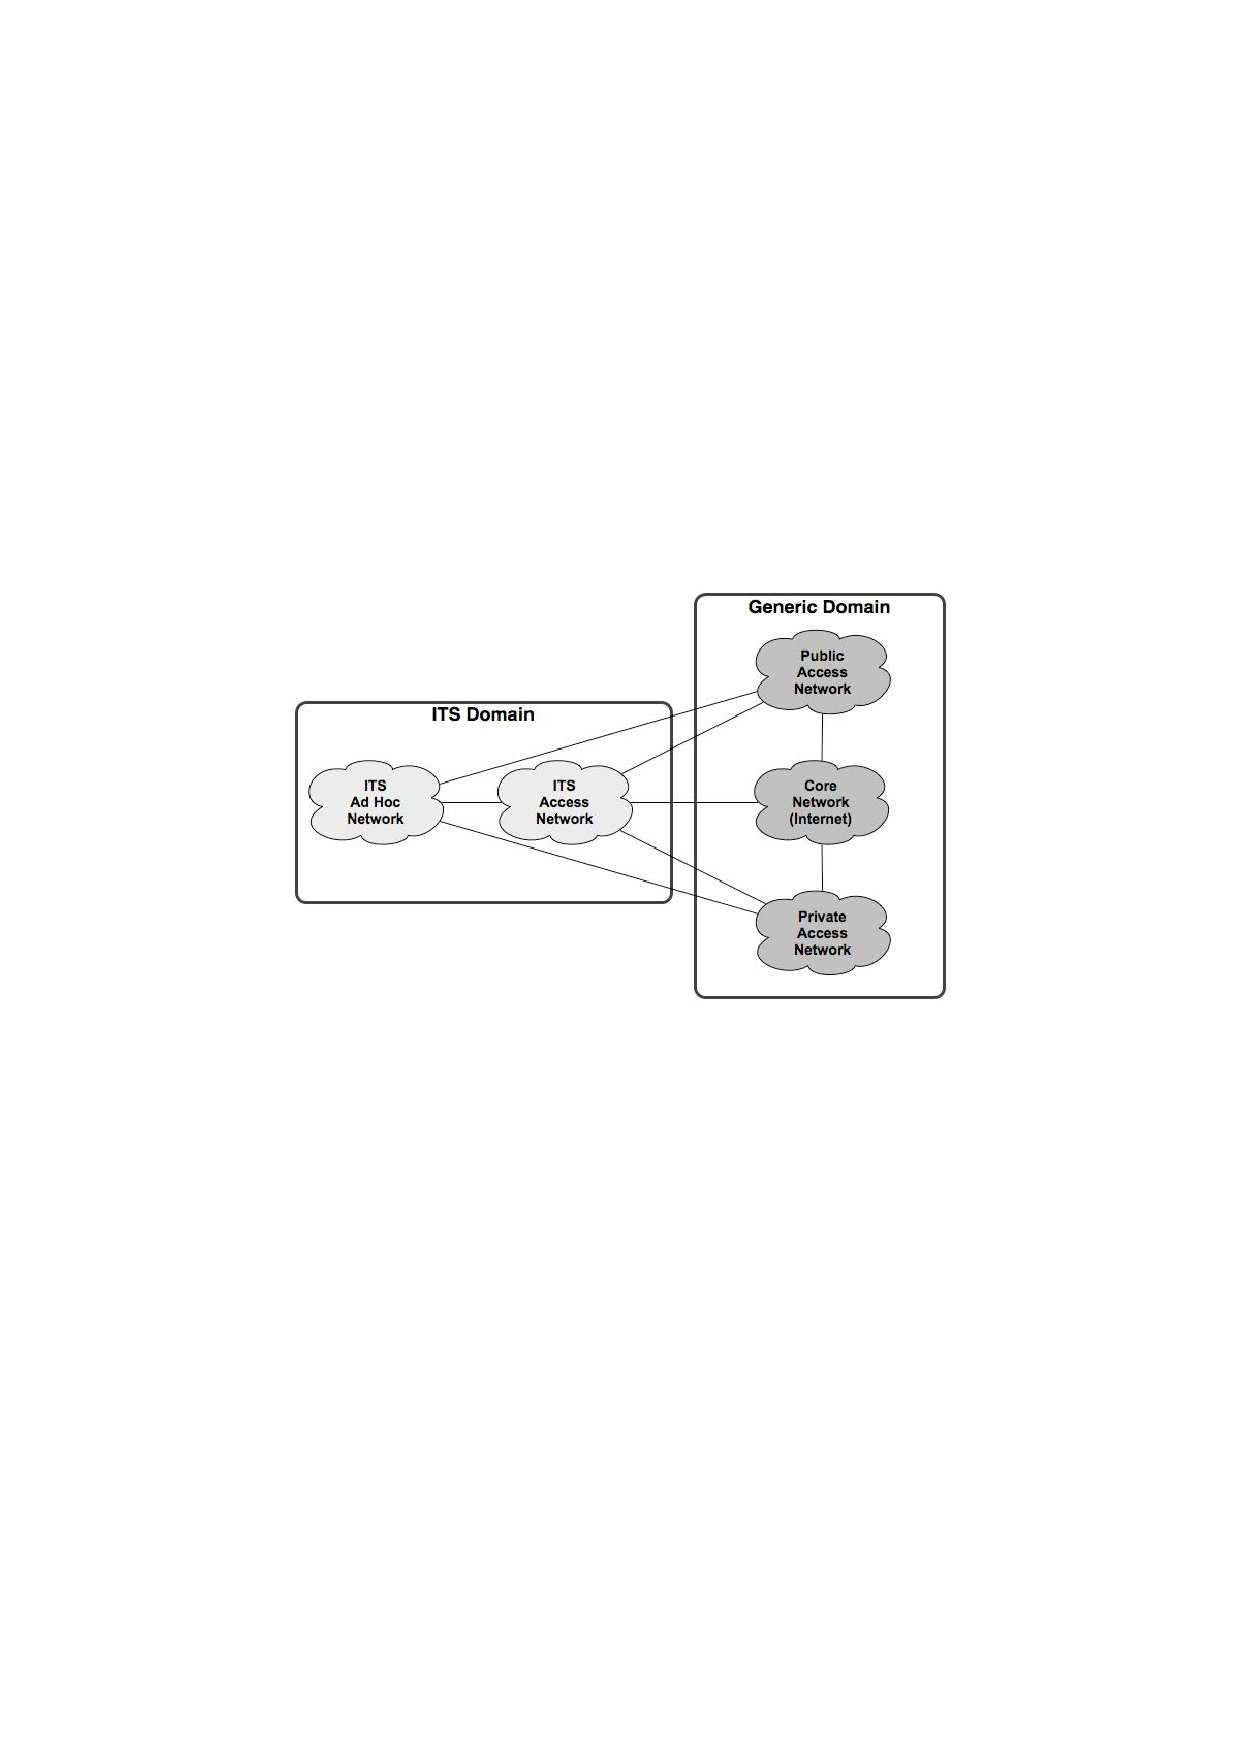
\includegraphics[width=0.99\textwidth]{content/images/02_architektur/uebersichtExterneNetzwerke.pdf}
	\caption{Überblick über die externen Netzwerke \cite{etsi302636-3}}
	\label{fig:architektur_ueberblickNetzwerke}
\end{figure}

\section{Übersicht über die verschiedenen Netzwerke \label{architektur_ueberblickNetzwerke}}
Dieser Abschnitt soll lediglich eine Übersicht über die verwendeten Netzwerke geben. Eine weitere Erklärung der Netzwerke findet an dieser Stelle nicht statt und ist nicht Gegenstand dieser Ausarbeitung. Die Netzwerke dürfen auch nicht isoliert betrachtet werden. Im Abschnitt \ref{funktionsweise_funktionaleKomponenten} wurden funktionale Komponenten mit Routingfunktionalitäten vorgestellt. Diese können die Netze und somit ihre Vorteile, bzw. ihre Dienste, miteinander verbinden.

Selbstverständlich benötigen die \ac{ITS} Stations Zugang zu einem der im Folgenden aufgeführten Netze. Der Zugang zum Core Network \ref{achitektur_coreNetwork} erfolgt über eins der anderen Netze. 

\subsection{ITS Ad Hoc Network\label{achitektur_adHocNetwork}}
Das \ac{ITS} Ad Hoc Netzwerk ist das Netzwerk für die Kommunikation zwischen \ac{IRS}, \ac{IVS} und \ac{PSS}. Die Kommunikation findet über die Luftschnittstelle statt. Sie ist in ihrer Reichweite begrenzt, dafür ist sie mobil einsetzbar. Die Drahtlose Kommunikation wird im Normalfall über den Standard ITS-G5 ermöglicht.


\subsection{ITS Access Network \label{architektur_itsAccessNetwork}}
\tocheck{Nicht die blasseste Ahnung ob das mit den Access Networks stimmt}
ITS Access Network werden zur Vernetzung von \ac{ITS} Komponenten verwendet. Diese Netzwerke bieten den Zugang für die entsprechenden \ac{ITS} Services. Sie werden als eigene Netzwerke realisiert. \ac{ITS} Stations werden durch Access Networks verbunden. Das bedeutet, dass \ac{IRS} untereinander über Access Networks verbunden sein können, es können aber auch Stations, die normalerweise Ad Hoc miteinander kommunizieren dieses Netz nutzen. 

\subsection{Public Access Network}
Ein Public Access Network ermöglicht den Zugang in öffentlich zugängliche Mehrzwecknetzwerke. Dieses Netzwerk kann beispielsweise dazu genutzt werden, um \ac{ITS} Stations mit dem Core Netzwerk zu verbinden. 

\subsection{Private Access Network}
Ein Private Access Network reguliert den Zugang durch die Teilnehmer. Die angebotenen Datendienste stehen nur einer bestimmten Gruppe von Nutzern zur Verfügung. Mit Private Access Networks besteht die Möglichkeit, eine gesicherte Verbindung in ein anderes Netzwerk aufzubauen. So kann beispielsweise ein \ac{IVS} auf das Intranet einer Firma zugreifen. 

\subsection{Core Network \label{achitektur_coreNetwork}}
Das Core Network ist ein Verbindungsnetz. Es hat keine \ac{ITS} Funktionalitäten und wird im Standard auch nicht weiter spezifiziert. Es wird in Verbindung mit den Public Access Network dazu genutzt, traditionelle Dienste, wie Internet oder Email, anzubieten.
 
\begin{figure}
	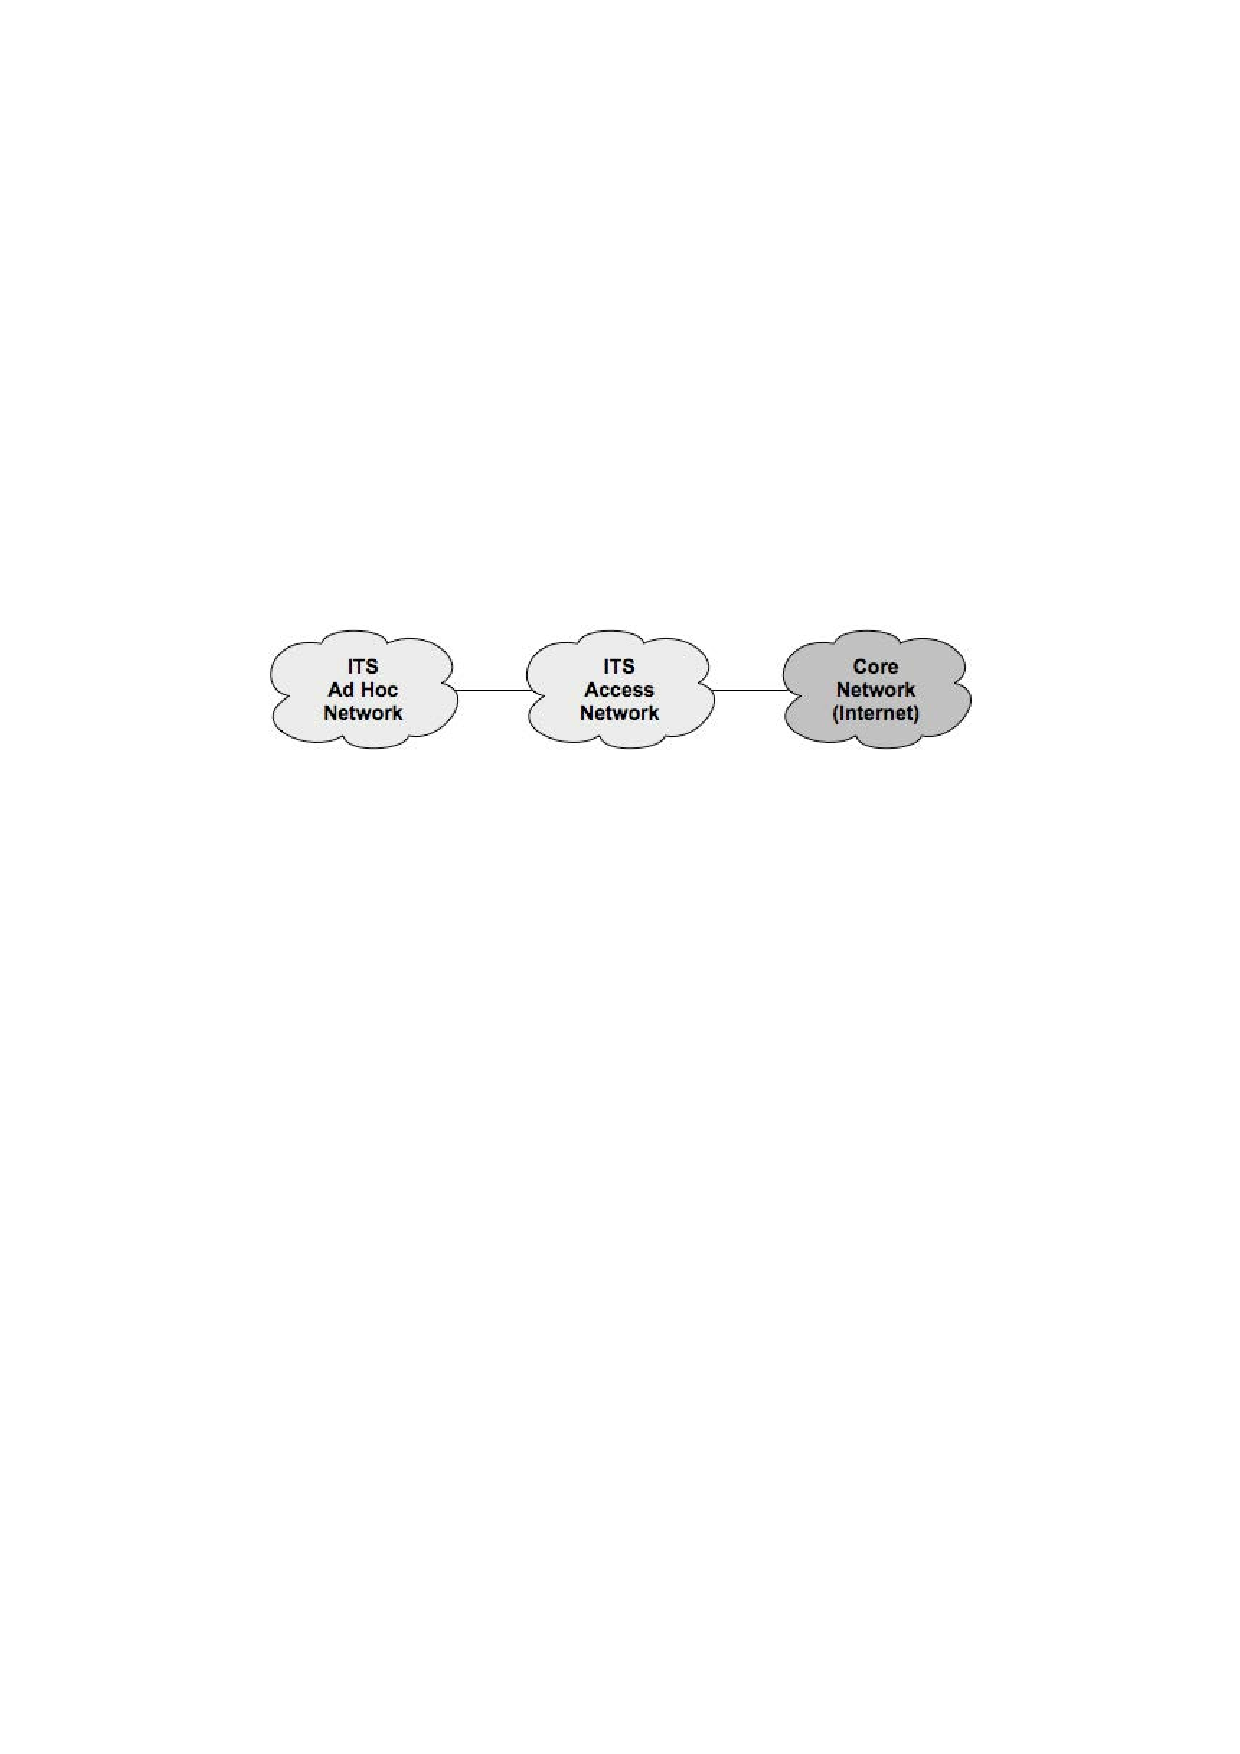
\includegraphics[width=0.75\textwidth]{content/images/02_architektur/netzwerkSzenario.pdf}
	%\vspace{2cm}
	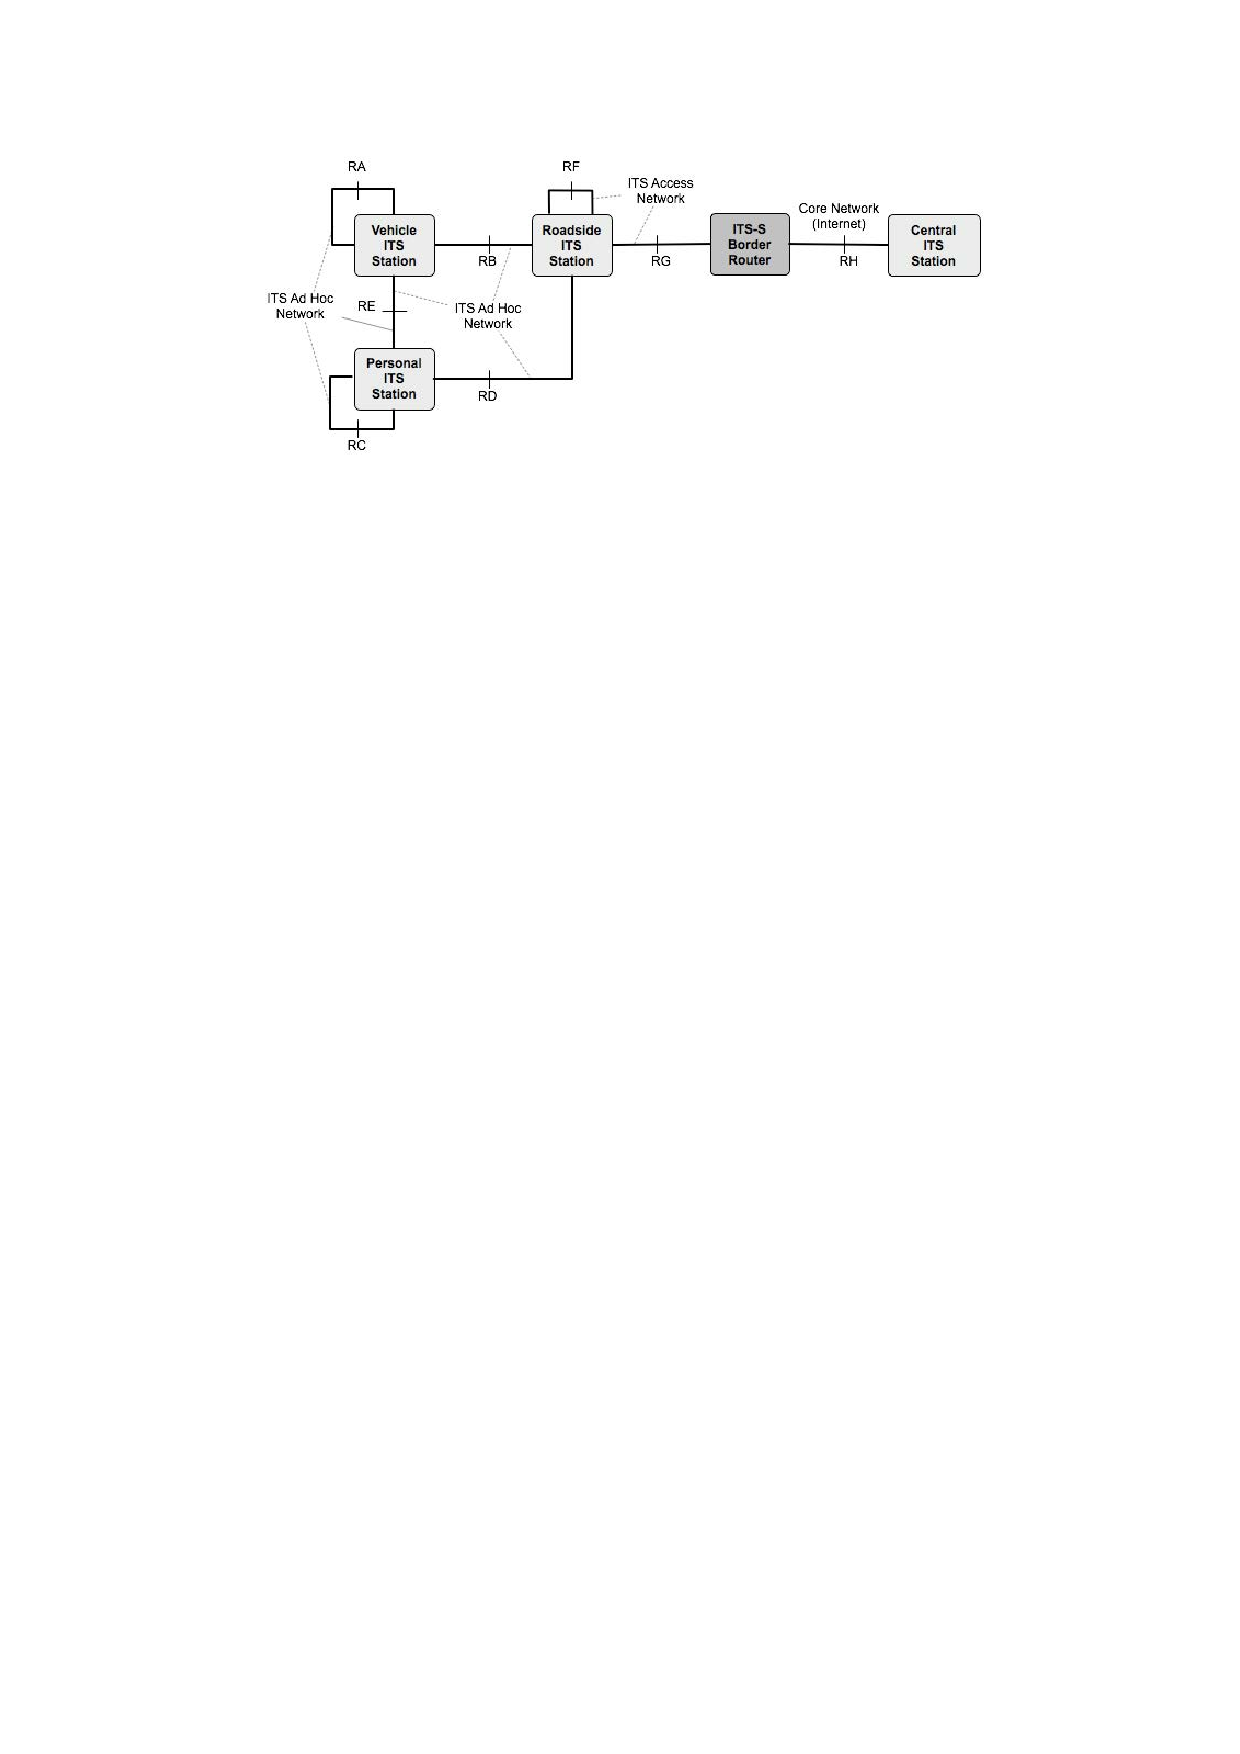
\includegraphics[width=0.75\textwidth]{content/images/02_architektur/verbindungenNetzwerkSzenario.pdf}
	\caption{Netzwerkszenario mit dazugehöriger Implementierung \cite{etsi302636-3}}
	\label{fig:architektur_netzwerkSzenario}
\end{figure}

Die Grafik \ref{fig:architektur_netzwerkSzenario} stammt aus dem Standard \cite{etsi302636-3}. Dort ist im oberen Teil der Grafik ein Szenario beschrieben, welche Netzwerke miteinander verbunden sein können.  Zu erkennen ist, dass die Netzwerke ITS Ad Hoc Netzwerk \ref{achitektur_adHocNetwork}, ITS Access Network \ref{architektur_itsAccessNetwork} und das Core Network  \ref{achitektur_coreNetwork} miteinander verbunden sein sollen.

Der untere Teil der Grafik zeigt eine Implementierungsmöglichkeit dieses Szenarios. Die hellen Rechtecke beschreiben die Komponenten, die in dieser Implementierung im System integriert sind, das dunkle Rechteck beschreibt die funktionale Komponente, die in diesem System beteiligt ist. Die Linien sind mit dem Typ des Netzwerks, welches sie repräsentieren beschriftet und zusätzlich mit dem Network Reference Point, den sie benutzen, beschriftet.
\todo{Sollen wir hier noch was zum Thema Network Reference Point schreiben? Ich glaube aber, dass die noch in den Layern kommen}


Auflistung und kurze Beschreibung der genutzten Network Reference Points:
\begin{itemize}
	\item \textbf{RA: } Reference Point zwischen \ac{IVS} über das ITS Ad Hoc Network
	\item \textbf{RB: } Reference Point zwischen \ac{IVS} und \ac{IRS} über das ITS Ad Hoc Network
	\item \textbf{RC: } Reference Point zwischen \ac{PSS} über das ITS Ad Hoc Network
	\item \textbf{RD: } Reference Point zwischen \ac{PSS} und \ac{IRS} über das ITS Ad Hoc Network
	\item \textbf{RE: } Reference Point zwischen \ac{IVS} und \ac{PSS} über das ITS Ad Hoc Network
	\item \textbf{RF: } Reference Point zwischen \ac{IRS} über das ITS Access Network
	\item \textbf{RG: } Reference Point zwischen \ac{IRS} und einem ITS-S Border Router \footnote{Der Border Router muss nicht explizit aufgeführt werden, da er als funktionale Komponente Teil einer Komponente ist. \label{ftn:borderRouter}} über das ITS Access Network 
	\item \textbf{RH: } Reference Point zwischen \ac{ICS} und ITS-S Border Router \footref{ftn:borderRouter} über das Core Network		
\end{itemize}

Erkennbar ist in dieser Implementierung, dass sich für mobile Stations Ad Hoc Netzwerke verwendet wurden. Diese haben den Vorteil, dass sie bereits in der Spezifikation mit der Luftschnittstelle ITS-G5 ausgestattet sind, was eine Mobilität erst ermöglicht. Was auch erkennbar ist, ist, dass die reinen ITS Netzwerke durch einen Border Router vom Core Network getrennt sind. Auch wenn hier nicht explizit aufgeführt, die \ac{ICS} benötigt in diesem Fall auch einen Border Router.

 
\section{ITS Station Reference Architecture}
\todo{komplette Section ITS Station Reference Architecture überarbeiten}
Eine Referenzarchitektur beschreibt ein allgemeines Modell einer Architektur. Das bedeutet, dass basierend auf dieser Architektur verschiedene Implementierungen existieren können. 

Die \ac{ITS} Station Reference Architecture unterscheidet sich grundlegend von bekannten Architekturen. Da sie während der Entwicklung an das \ac{OSI} Modell angelehnt war, ergeben sich einige Parallelen:
\begin{itemize}
	\item Trennung der einzelnen Layer
	\item Definition von Service Primitiven zwischen den Layern
	\item Die Standards beziehen die Layer auf die \ac{OSI} Layer. 
\end{itemize}

Der direkte Vergleich mit dem \ac{OSI} Modell und die Zuordnung der Layer wird in \autoref{fig:architektur_vergleichItsOsi} deutlich.

\begin{figure}[h]
	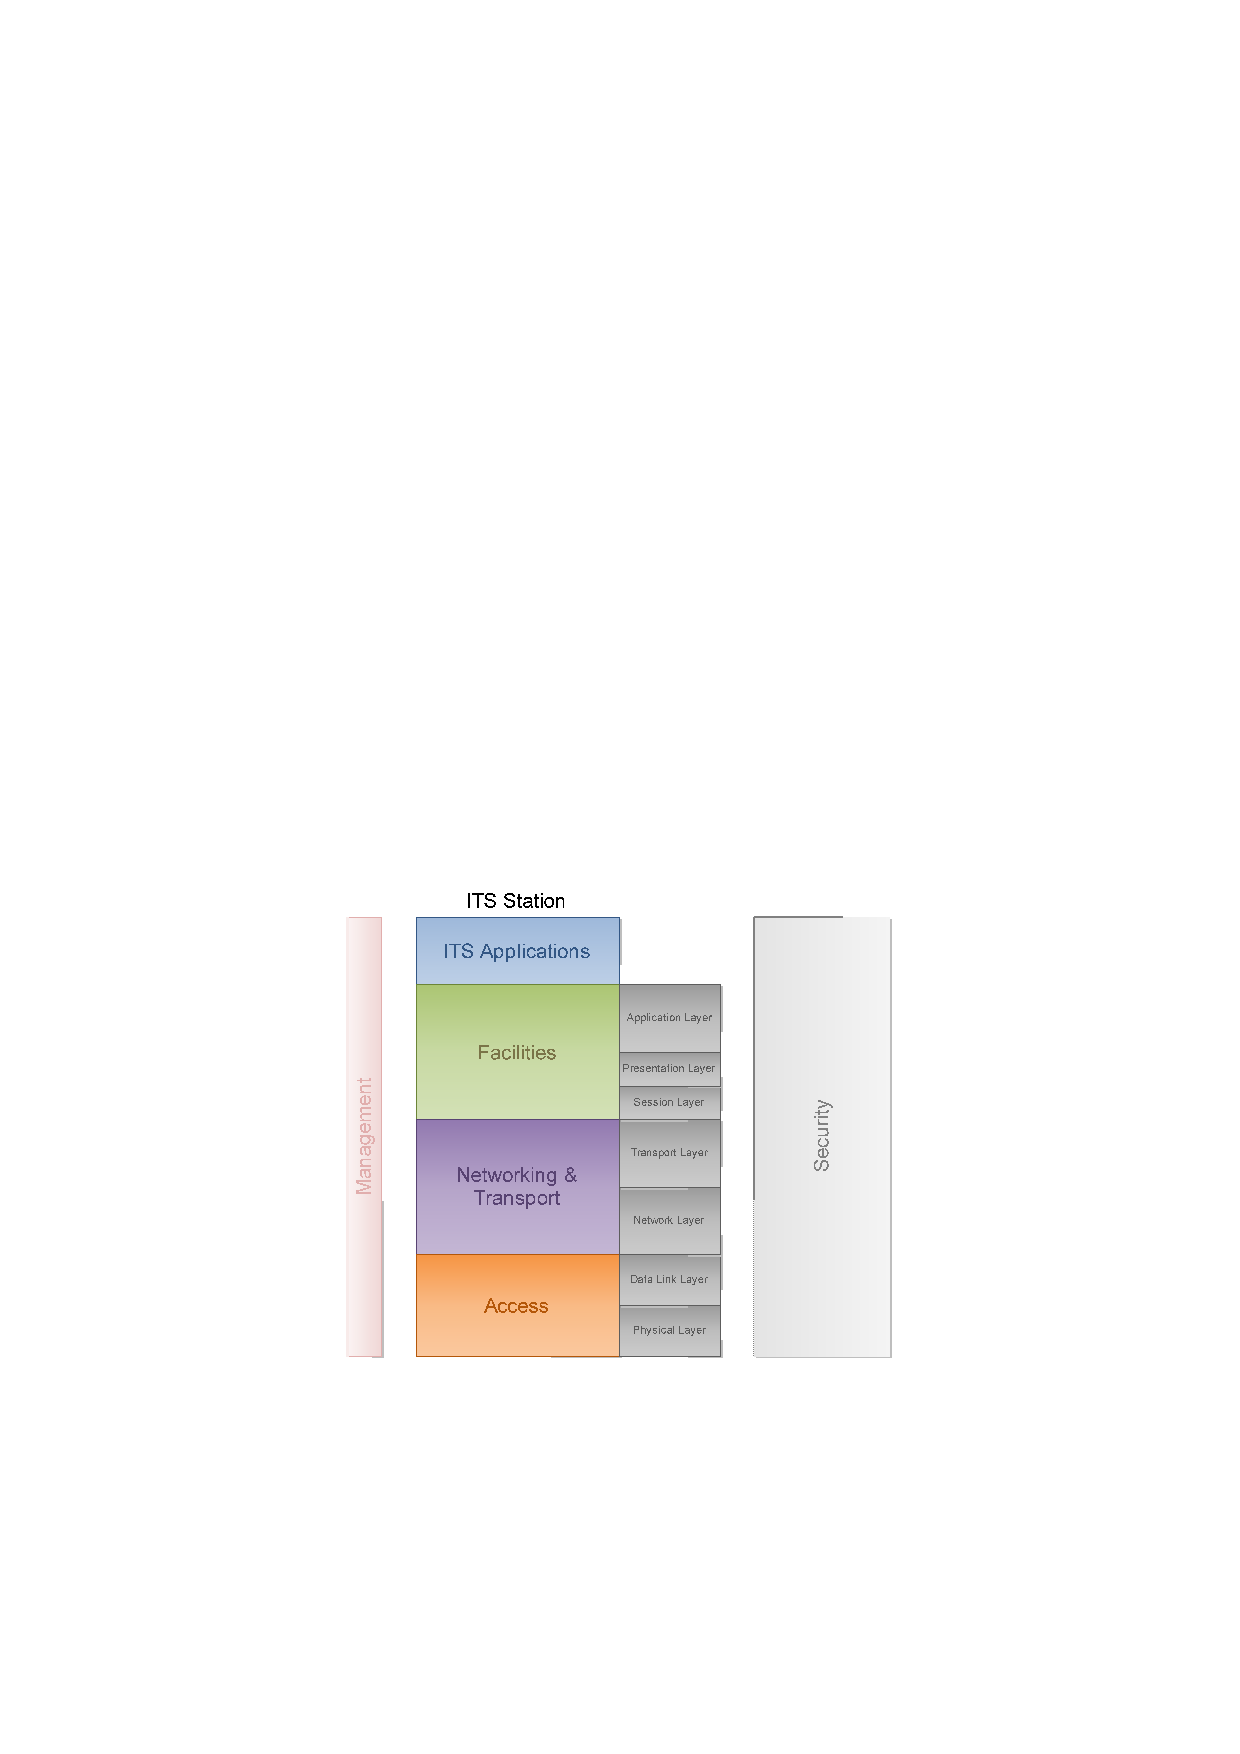
\includegraphics[width=0.99\textwidth]{content/images/02_architektur/vergleichITS-OSI.pdf}
	\caption{Der Vergleich zwischen ITS und OSI \cite{ts102940}}
	\label{fig:architektur_vergleichItsOsi}
\end{figure}

Obwohl das \ac{ITS} Station Reference Protocol bei der Entwicklung an das \ac{OSI} Modell angelehnt wurde gibt es jedoch einen gravierenden Unterschied: In der \ac{ITS} Station Reference Architecture sind Cross Layer vorgesehen. Das \ac{OSI} Referenzmodell ist wasserfallartig aufgebaut. Das bedeutet, dass die einzelnen Layer übereinander angeordnet sind. Jeder Layer hat jeweils nur zu dem direkt über- und unterliegenden Layer eine Schnittstelle. Cross Layer sind Layer, die in mehrere dieser Schichten Schnittstellen haben. Sie erweitern die vorhanden Layer in horizontaler Richtung. Im Fall der \ac{ITS} Station Reference Architecture sind das die Layer \glqq Management\grqq~ und \glqq Security\grqq. Sie haben Schnittstellen, bzw. Primitiven in alle anderen Layer. 

\begin{figure}
	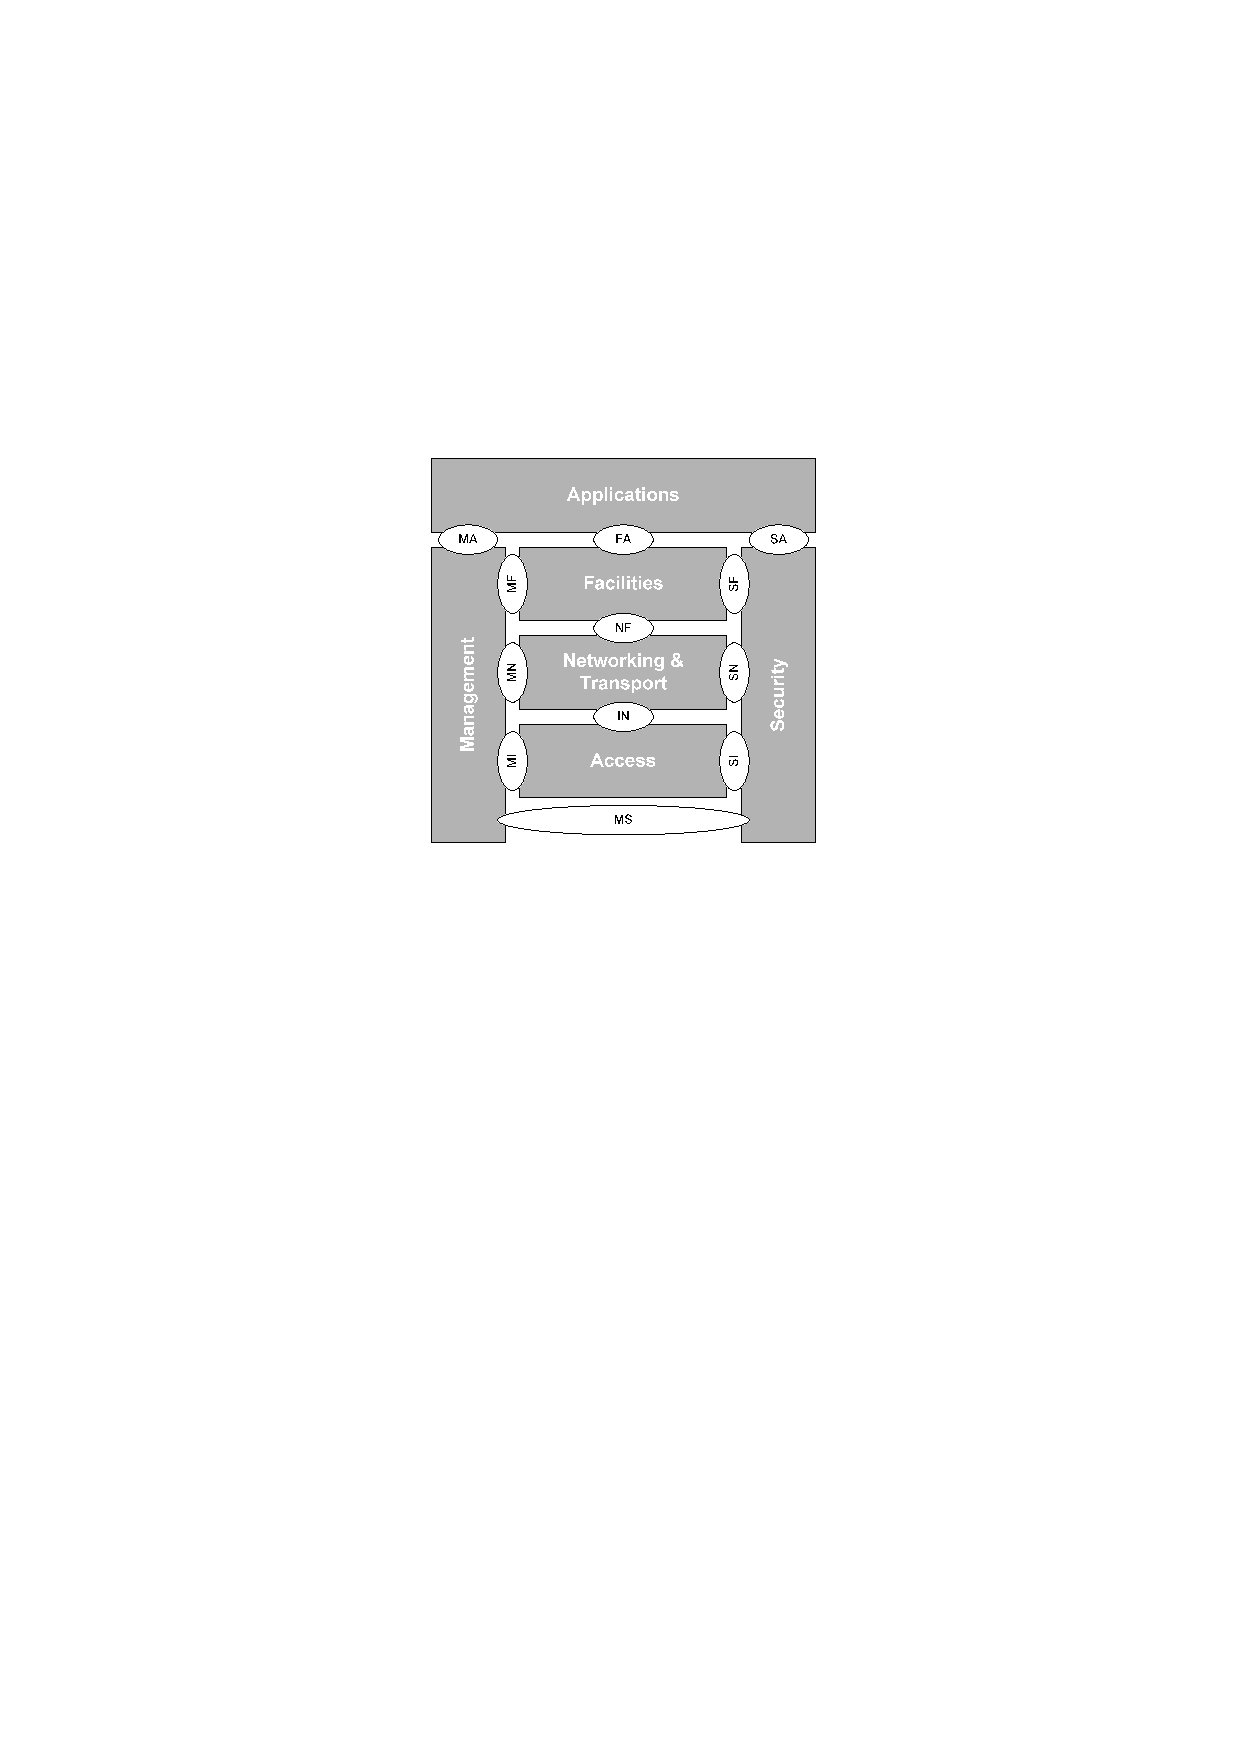
\includegraphics[width=0.75\textwidth]{content/images/02_architektur/stationReferenceArchitecture.pdf}
	\caption{Darstellung der ITS Station Reference Architecture \cite{ts102940}}
	\label{fig:funktionsweise_referenceArchitecture}
\end{figure}

\section{Horizontal Layer}
Dieser Abschnitt beschreibt die Layer, die klassisch übereinander angeordnet sind. Die Layer und ihre Funktionen entsprechen den Layern des \ac{OSI} Modells. Sie sind aber anders aufgeteilt.

\subsection{Access}
\todo{Noch etwas über die Channel herausfinden und schreiben}
Der Access Layer von ITS entspricht den \ac{OSI} Layern 1 und 2. Er besteht aus zwei Subaltern und hat drei Interfaces, bzw. \ac{SAP}. Die Sublayer sind der \glqq Data Link Layer (DLL)\grqq~und der \glqq Physical Layer (PHY)\grqq. Der DLL kann weiter in den \glqq Medium Access Control (MAC)\grqq~und den \glqq Logical Link Control (LLC)\grqq~Layer unterteilt werden. Zusätzlich zu den Subalayern hat der Access Layer ein Layer Management. Dieses verwaltet die Sublayer. Es arbeitet nur nur im Access Layer und darf nicht mit dem  Management Layer \ref{architektur_managementLayer} verwechselt werden.

Die \ac{SAP} sind:
\begin{itemize}
	\item \textbf{SAP-IN: } Als \ac{SAP} zu dem nächst höheren Layer  Networking \& Transporting \ref{architektur_networkingTransporting}
	\item \textbf{SAP-SI: } Als \ac{SAP} zu dem Cross Layer Security Layer \ref{architektur_securityLayer}
	\item \textbf{SAP-MI: } Als \ac{SAP} zu dem Cross Layer Management Layer \ref{architektur_managementLayer}
\end{itemize}
\todo{ISO 21217 finden - Scheinbar infos über die Layer}

\todo{mal in ETSI TS 102 723-10 reinsehen, ob da was interessantes zu den SAP drin steht}

Der Access Layer ist nicht auf ein bestimmtes Übertragungsprotokoll festgelegt. Beispiele für ein Übertragungsprotokoll sind ITS-G5, WiFi, BlueTooth, Ethernet\dots In einer reinen \ac{C2C} Kommunikation bietet sich aber vor allem ITS-G5 an, für eine allgemeine \ac{ITS} Verbindung haben die anderen Übertragungsprotokolle aber auch ihre Berechtigung. Diese Übertragungsprotokolle müssen aber den \ac{ITS} Protokollstack transparent übertragen. 

Der folgende Abschnitt beschreibt den Access Layer und legt G5 zugrunde.
 
\begin{figure}
	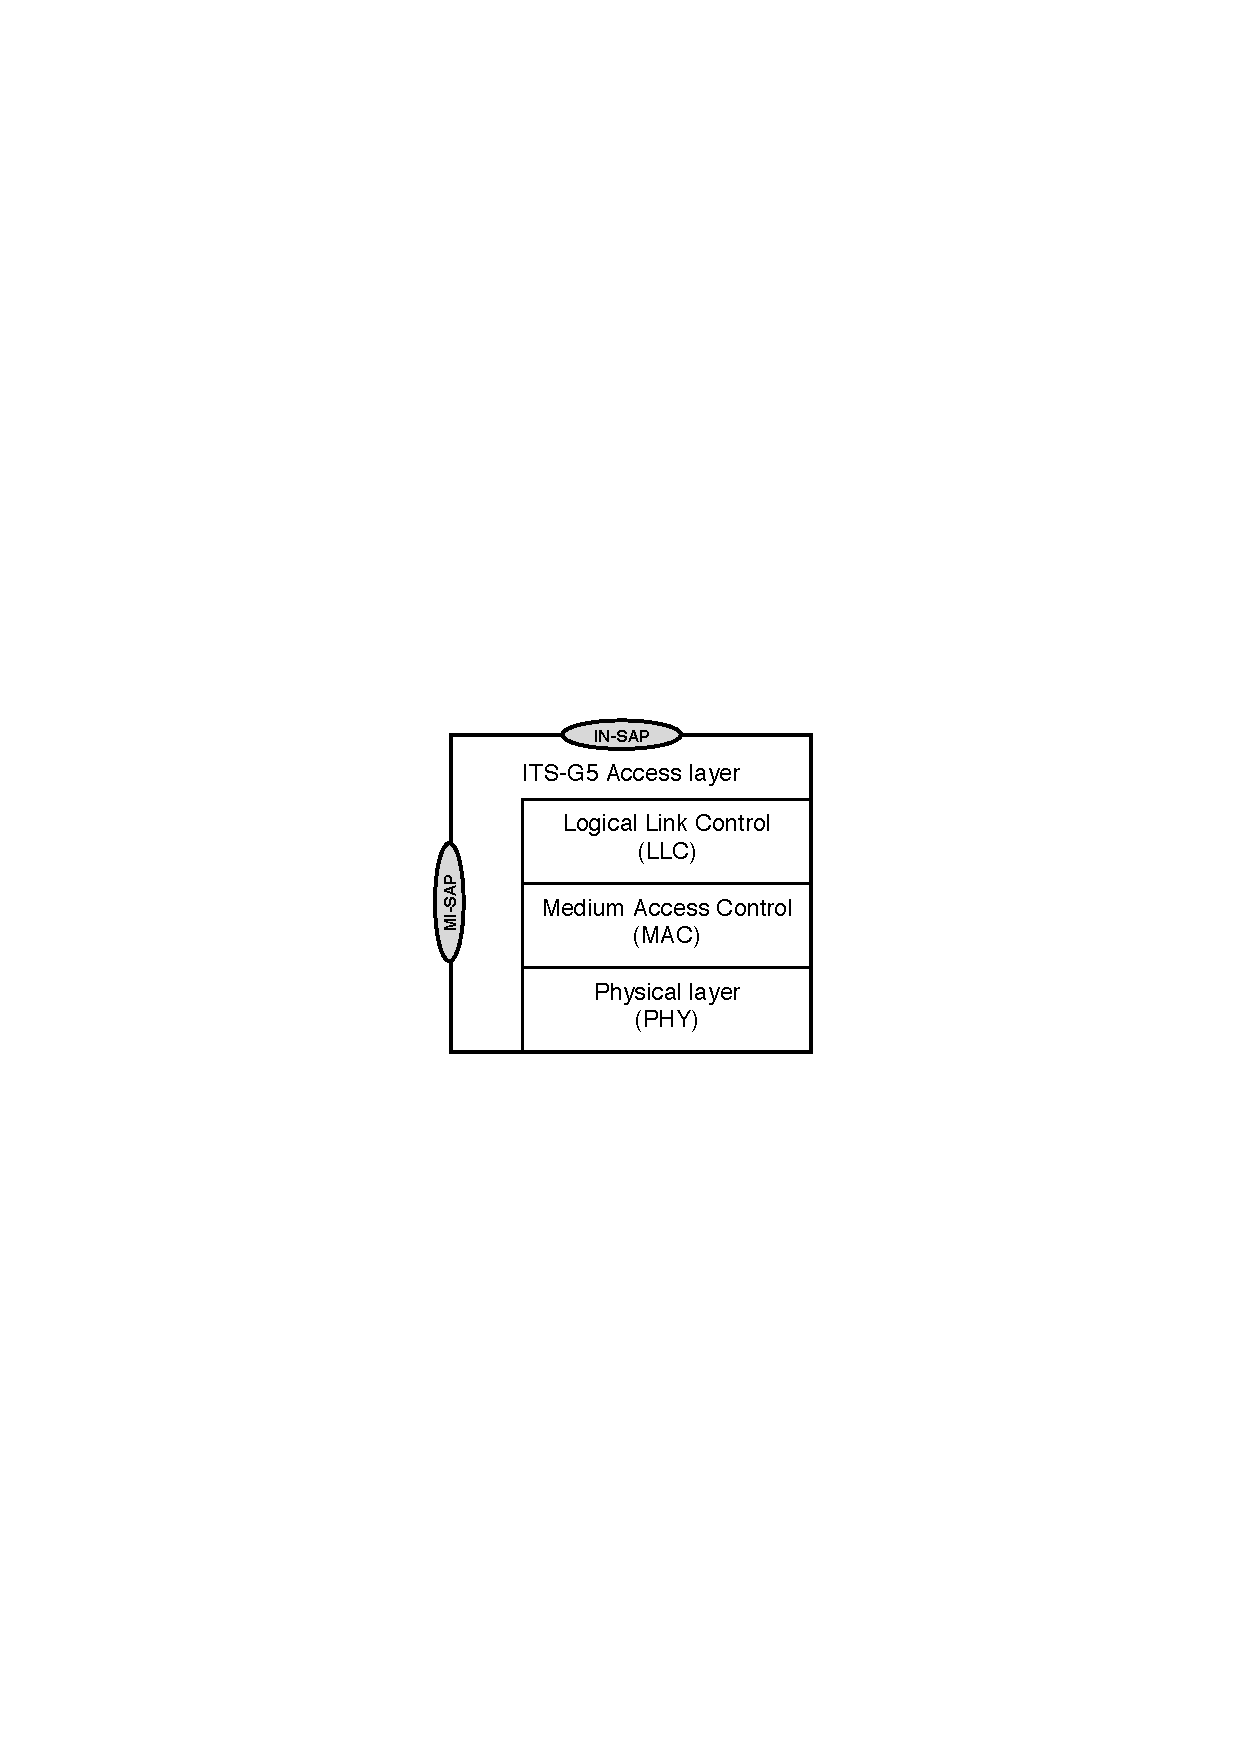
\includegraphics[width=0.75\textwidth]{content/images/02_architektur/accessLayer.pdf}
	%\missingfigure{Access Layer Bild noch aus dem Standard 302 665 herauskopieren }
	\caption{Darstellung des ITS G5 Access Layers \\cite{en302665}}
	\label{fig:architektur_accessLayer}
\end{figure}

Die Grafik \ref{fig:architektur_accessLayer} entspricht des untersten Layer der Grafik \ref{fig:funktionsweise_referenceArchitecture}. In der Grafik ist zu erkennen, dass der Access Layer drei Interfaces besitzt. Er hat Interfaces zu den Cross Layern und dem Network \& Transport Layer.


Im Access Layer finden eine Periodisierung und eine Aufteilung des Datenverkehrs in Logic Channels statt. Diese Aufgaben werden mit verschiedenen Ansätzen gelöst. Deswegen sind sie keinem Sublayer genau zuzuordnen, sondern müssen in der Beschreibung der Sublayer gesondert betrachtet werden.


Eine Funktion des Access Layers ist das im Abschnitt \ref{architektur_dcc} beschriebene \ac{DCC}. Hier finden die Mechanismen Transmit Power Control (TPC), \ac{DCC} sensitivity control (DSC), Transit rate control (TRC), transmit datarate control (TDC) und DCC access control (TAC) statt. TPC regelt die Auslastung der Kanäle. Dazu werden Grenzen definiert, die TPC überwacht und einhält. TRC überwacht die Zeiten von Datenpaketen. Dazu gehören beispielsweise die Latenz eines Pakets aber auch die Intervalle zwischen Paketen. TDC überwacht die reine Datenrate eines Channels. Dabei wird nicht nur die maximale Datenrate überwacht, es wird auch beispielsweise die minimale Datenrate überwacht. DSC überwacht, ob der Sender bereit zum Senden ist. Dazu wird anhand von definierten Grenzwerten gemessen, ob der Sender am Senden ist oder nicht. TAC regelt den Kanalzugriff. \todo{Kanalzugriff erklären, wenn ich weiß, was Kanäle sind. Quelle für TAC: \cite{etsi102687}}

\subsubsection{Physical Layer (PHY)}
Der Physical Sublayer verbindet physikalisch zu dem Kommunikationsmedium.

\subsubsection{Data Link Layer (DLL)}
Der Data Link Sublayer kann wiederum in den Medium Access Control (MAC) Sublayer und den Logical Link Control (LLC) Sublayer aufgeteilt werden. Der MAC Sublayer regelt den Zugriff auf das Kommunikationmeduim.


\ac{ITS} bietet die Funktionalität von logischen Kanälen. 




\subsection{Networking \& Transporting \label{architektur_networkingTransporting}}
Der Networking \& Transporting Layer enthält mehrere verschiedene Netzwerk und Transport Protokolle und entspricht den \ac{OSI} Layern 3 und 4. Die Aufgabe ist das Routing und der Ende zu Ende Transport von Daten. Er wird im Kapitel \ref{chap:networklayer} genauer beschrieben. 


\subsection{Facilities}
Der Facilities Layer entspricht den \ac{OSI} Layern 5, 6 und 7. Er bietet eine Sammlung von Funktionen, die die \ac{ITS} Anwendungen unterstützen. Der Layer bietet Datenstrukturen um verschiedene Date zu speichern, zu sammeln und zu verwalten. Er wird im Kapitel \ref{chap:facilitylayer} genauer erklärt.

\subsection{Applications}
Im Applications Layer werden die Use Cases realisiert. Ihnen steht der \ac{ITS} Protokoll Stack zu Verfügung. Eine genauere Beschreibung des Application Layers findet im Kapitel \ref{chap:applicationlayer} statt.

\section{Cross/Vertical Layer}
Die Cross Layer weichen stark vom \ac{OSI} Modell ab. Sie erweitern die traditionellen Layer, die jeweils nur ein Interface zum nächst höheren, bzw. tieferen Layer haben um Layer, die Interfaces zu allen anderen Layern haben. Durch die Interfaces zu allen Layern ergeben sich neue Möglichkeiten. So kann beispielsweise im Application Layer die genutzte Bandbreite an die im Physical Layer zur Verfügung stehende Bandbreite angepasst werden. Dadurch werden Überlastungen, die sich auf die Latenz auswirken oder zu fehlerhaften Übertragungen führen bereits im im Vorfeld vermieden.

\subsection{Management Layer \label{architektur_managementLayer}}
Der Management Layer übernimmt Alle Aufgaben, die mit der Verwaltung einer \ac{ITS} Station und deren Protokollstack zusammenzufassen sind. Vereinfacht gesagt verwaltet er im Protokollstack die Cross Layer Funktionalität. 


\begin{figure}
	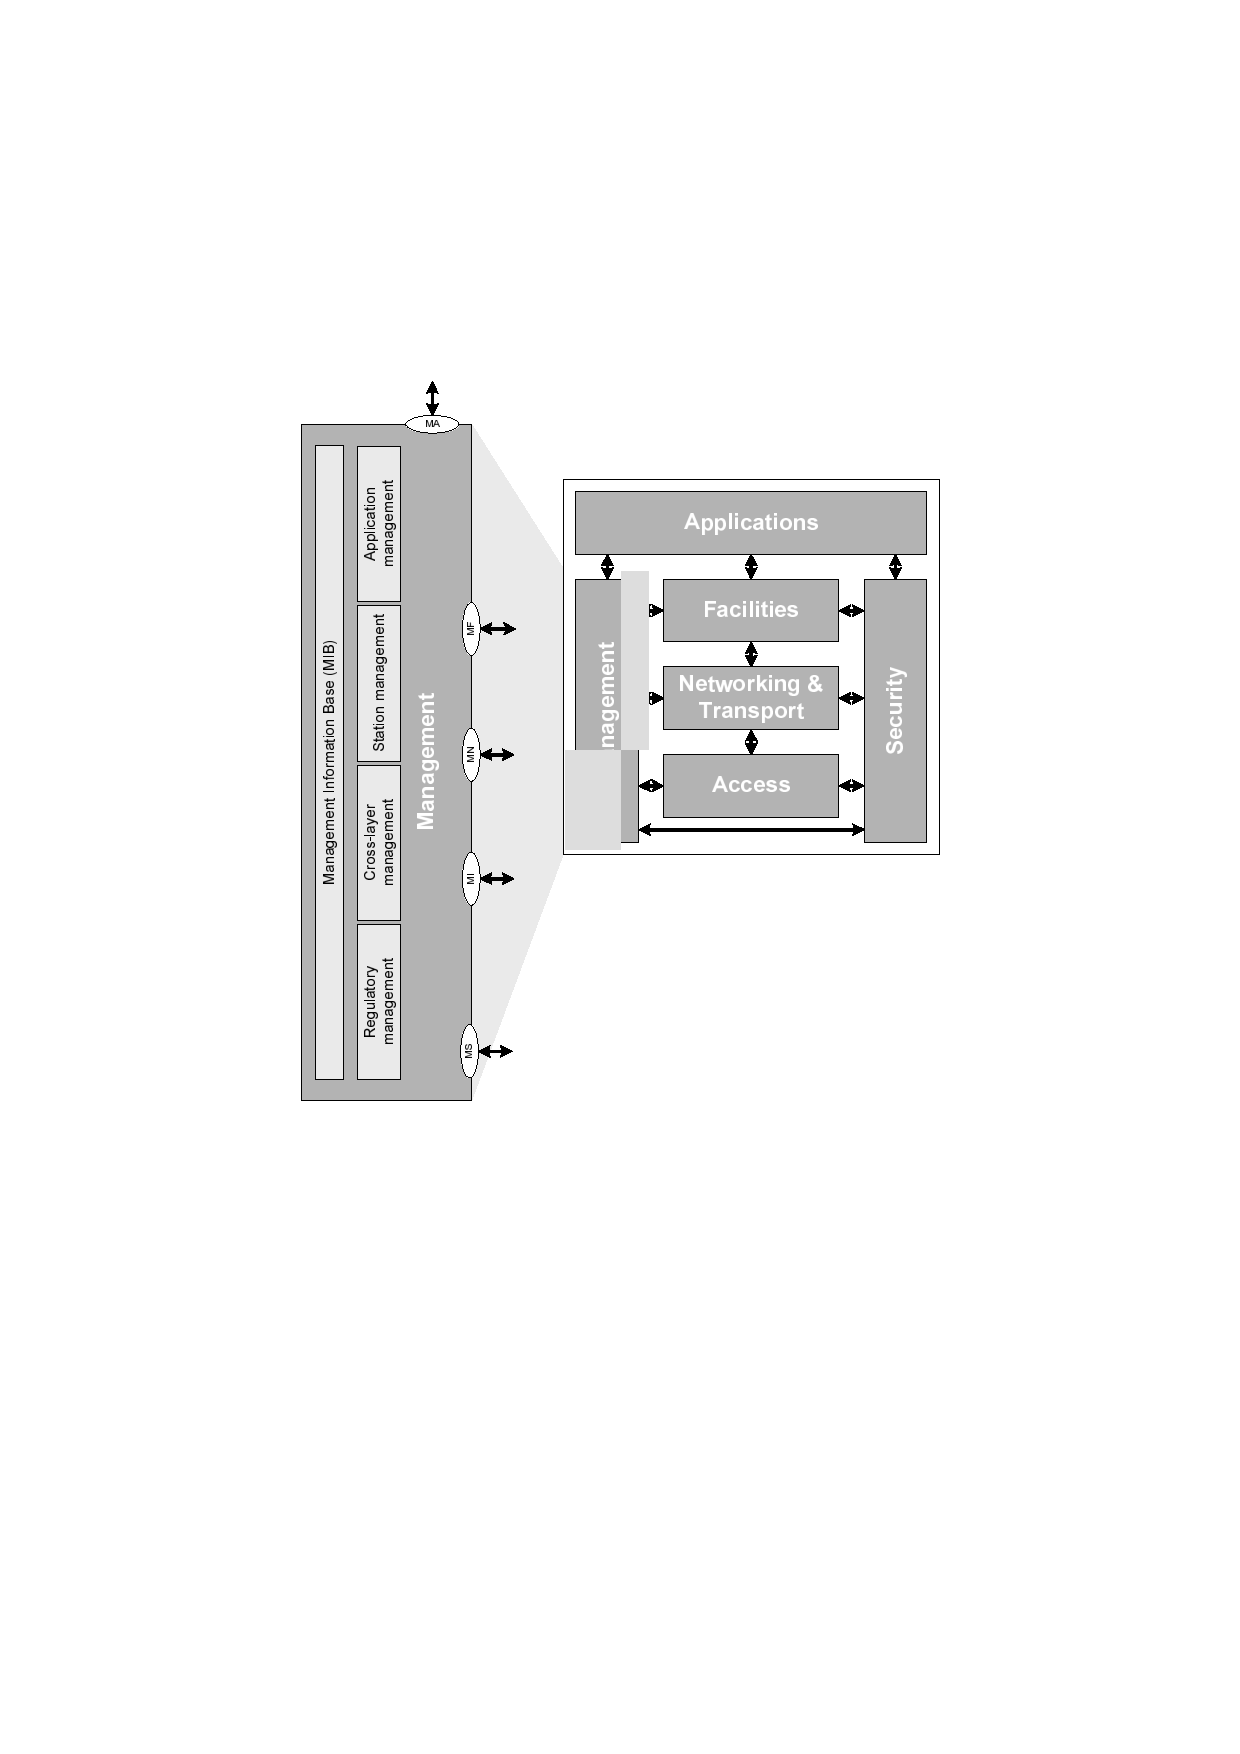
\includegraphics[width=0.75\textwidth]{content/images/02_architektur/managementLayer.pdf}
	\caption{Der Management Layer im Überblick \cite{etsi2010302}}
	\label{fig:architektur_managementLayer}
\end{figure}
\todo{Einzelne Untereinheiten der Grafik erklären, schreiben wo die beschriebenen Dienste angesiedelt sind}
In der  \autoref{fig:architektur_managementLayer} ist der Management Layer mit seinen Interfaces und Untereinheiten dargestellt. Er hat zu jedem anderen Layer ein Interface. Die fünf Untereinheiten ergeben sich aus den definierten Funktionalitäten des Management Layers. Die folgende Auflistung der Funktionalitäten ist dem Standard \cite{etsi2010302} entnommen:

\begin{itemize}
	\item Cross-interface Management
	\item Kommunikation zwischen Einheiten gem. ETSI TS 102 723-1
	\item Netzwerkmanagement
	\item Kommunikationsservice Management
	\item \ac{ITS} Anwendungs Management
	\item Station Management
	\item Management der allgemeinen Congestion Control
	\item Management des Service Advertisement
	\item Management des Systemschutzes 
	\item Eine alleine Informationsbasis
	\item Die Möglichkeit die verschiedenen Layer zu verbinden
\end{itemize}

\subsubsection{ITS Service Advertisement}
\ac{ITS} Service Adverticement ist der Mechanismus, mit dem eine \ac{ITS} Station \ac{ITS} Services erkennen kann. Bei diesem Mechanismus macht eine \ac{ITS} Station, in dem Fall der Service Provider, aktiv ihre Services anderen \ac{ITS} Stations, in dem Fall Service User, bekannt. Eine Möglichkeit, die Services bekannt zu machen ist das FAST Service Advertisement. Es ist im Standard ISO/IEC 24102 definiert und eignet sich für die Luftschnittstelle mit lediglich einem Hop. Beim FAST Service Advertisement wird ein Advertisement Manager benötigt. Dieser empfängt die Service Adverticements von den anderen Service Providern und sendet die Service Adverticements der eigenen \ac{ITS} Station in regelmäßigen Abständen aus.

Für das Aussenden von Service Advertisements gibt es \ac{SAM}. \autoref{architektur_darstellungSAMHeader} zeigt den Aufbau einer \ac{SAM}. Sie besteht aus einem Header und einem Body. Der Header enthält die Elemente:

\begin{itemize}
	\item samID: Identifiziert die \ac{SAM}
	\item Version: Die Versionsnummer der \ac{SAM}
	\item stationID: Die ID des sendenden Service Providers
\end{itemize}

Der Body enthält die folgenden Elemente:
\begin{itemize}
	\item serviceList: Eine Liste mit den angebotenen Services. Sie sind nach dem Standard ISO 17419 eindeutig kodiert
	\item channelList:  Eine Information, welche Channels für die Service Operation Phase genutzt werden
	\item ipServList: Informationen über Services, die angeboten wurden und der Service Operation Phase IPv6 benötigen.
\end{itemize} 


\begin{figure}[h]
	\begin{bytefield}{40}
		\wordbox{1}{Service Advertisement Message SAM} \\
		\bitbox{16}{Header} & \bitbox{24}{Body} \\
		\bitbox{4}{samID} & \bitbox{4}{Version} & \bitbox{8}{stationID} & \bitbox{8}{serviceList} & \bitbox{8}{channelList} & \bitbox{8}{ipServList}
		\end{bytefield}
	\caption{Darstellung eines SAM Pakets}
	\label{architektur_darstellungSAMHeader}
\end{figure}

Der Service User beantwortet die \ac{SAM} mit einer \ac{CTX}. Die \ac{CTX} ist ähnlich aufgebaut wie die \ac{SAM}. In der \autoref{architektur_darstellungCTXHeader} ist eine \ac{CTX} dargestellt.

\begin{figure}[h]
	\begin{bytefield}{32}
		\wordbox{1}{Context Message CTX} \\
		\bitbox{16}{Header} & \bitbox{16}{Body} \\
		\bitbox{4}{ctxID} & \bitbox{4}{Version} & \bitbox{8}{clientID} & \bitbox{8}{servContext\-List} & \bitbox{8}{ipContext\-List}
		\end{bytefield}
	\caption{Darstellung eines CTX Pakets}
	\label{architektur_darstellungCTXHeader}
\end{figure}

Der Header der \ac{CTX} entspricht dem einer \ac{SAM}. Hier wird aber anstatt der \ac{ID} des Providers die \ac{ID} des Clients mitgesendet. Im Body unterscheiden sich die Nachrichten. 

Die Body Inhalte einer \ac{CTX}:
\begin{itemize}
	\item servContextList: Informationen über den Service Kontext, der beim Service User verfügbar ist. Kann als Antwort auf einen angebotenen Service in der serviceList der \ac{SAM} vorliegen.
	\item ipContextList: Informationen über Service Kontexte, die beim Service User verfügbar sind und IPv6 benötigen. Kann als Antwort auf einen Service, der in der ipServList der \ac{SAM} angeboten wurde vorliegen.
\end{itemize}  

Das Bekanntmachen von Services kann auf zwei Arten erfolgen. Die Möglichkeiten unterscheiden sich darin, dass bei der ersten Möglichkeit die \ac{SAM} vom Service User mit einer \ac{CTX} beantwortet wird. Bei der zweiten Möglichkeit wird die \ac{SAM} nicht beantwortet. Grundsätzlich laufen die Möglichkeiten aber gleich ab.  

Die Kommunikation zwischen User und Provider kann man in zwei Phasen aufteilen. Die Service Initialization Phase und die Service Operation Phase.

Der Zweck der Service Invitation Phase ist es die Session aufzubauen. Dabei wird der Service User mit einer \ac{SAM} eingeladen. Während der Service Invitation Phase wird zwischen den beschriebenen Möglichkeiten unterschieden. Ob eine \ac{SAM} von einer \ac{CTX} bestätigt wird, hängt davon ab, ob es sich beim Service User um eine \ac{ITS} application class oder eine \ac{ITS} application handelt. Der Unterschied zwischen \ac{ITS} Application Class und \ac{ITS} Application ist, dass von einem Application Objekt mehrere Kontexte existieren können. Jeder Kontext kann auf eine \ac{ITS} Application referenziert werden. Bei der Übertragung wird der Unterschied durch  den \ac{ASN.1} Typ \glqq DSRCapplicationEntityID\grqq~als Markierung deutlich gemacht. 

Bei der Einladung von Application Classes wird die \ac{SAM} durch eine \ac{CTX} bestätigt. Bei Applications wird keine \ac{CTX} versendet. Die Service Invitation Phase wird als erfolgreich angesehen, sobald das erste \glqq REQUW\grqq~oder \glqq REQN\grqq~versendet wird. 

Nach der erfolgreichen Service Invitation Phase folgt die Service Operation Phase. \todo{rausfinden, was in dieser Phase statt findet}
\begin{figure} 
  \centering 
   \subfigure[Ohne Bestätigung durch CTX] {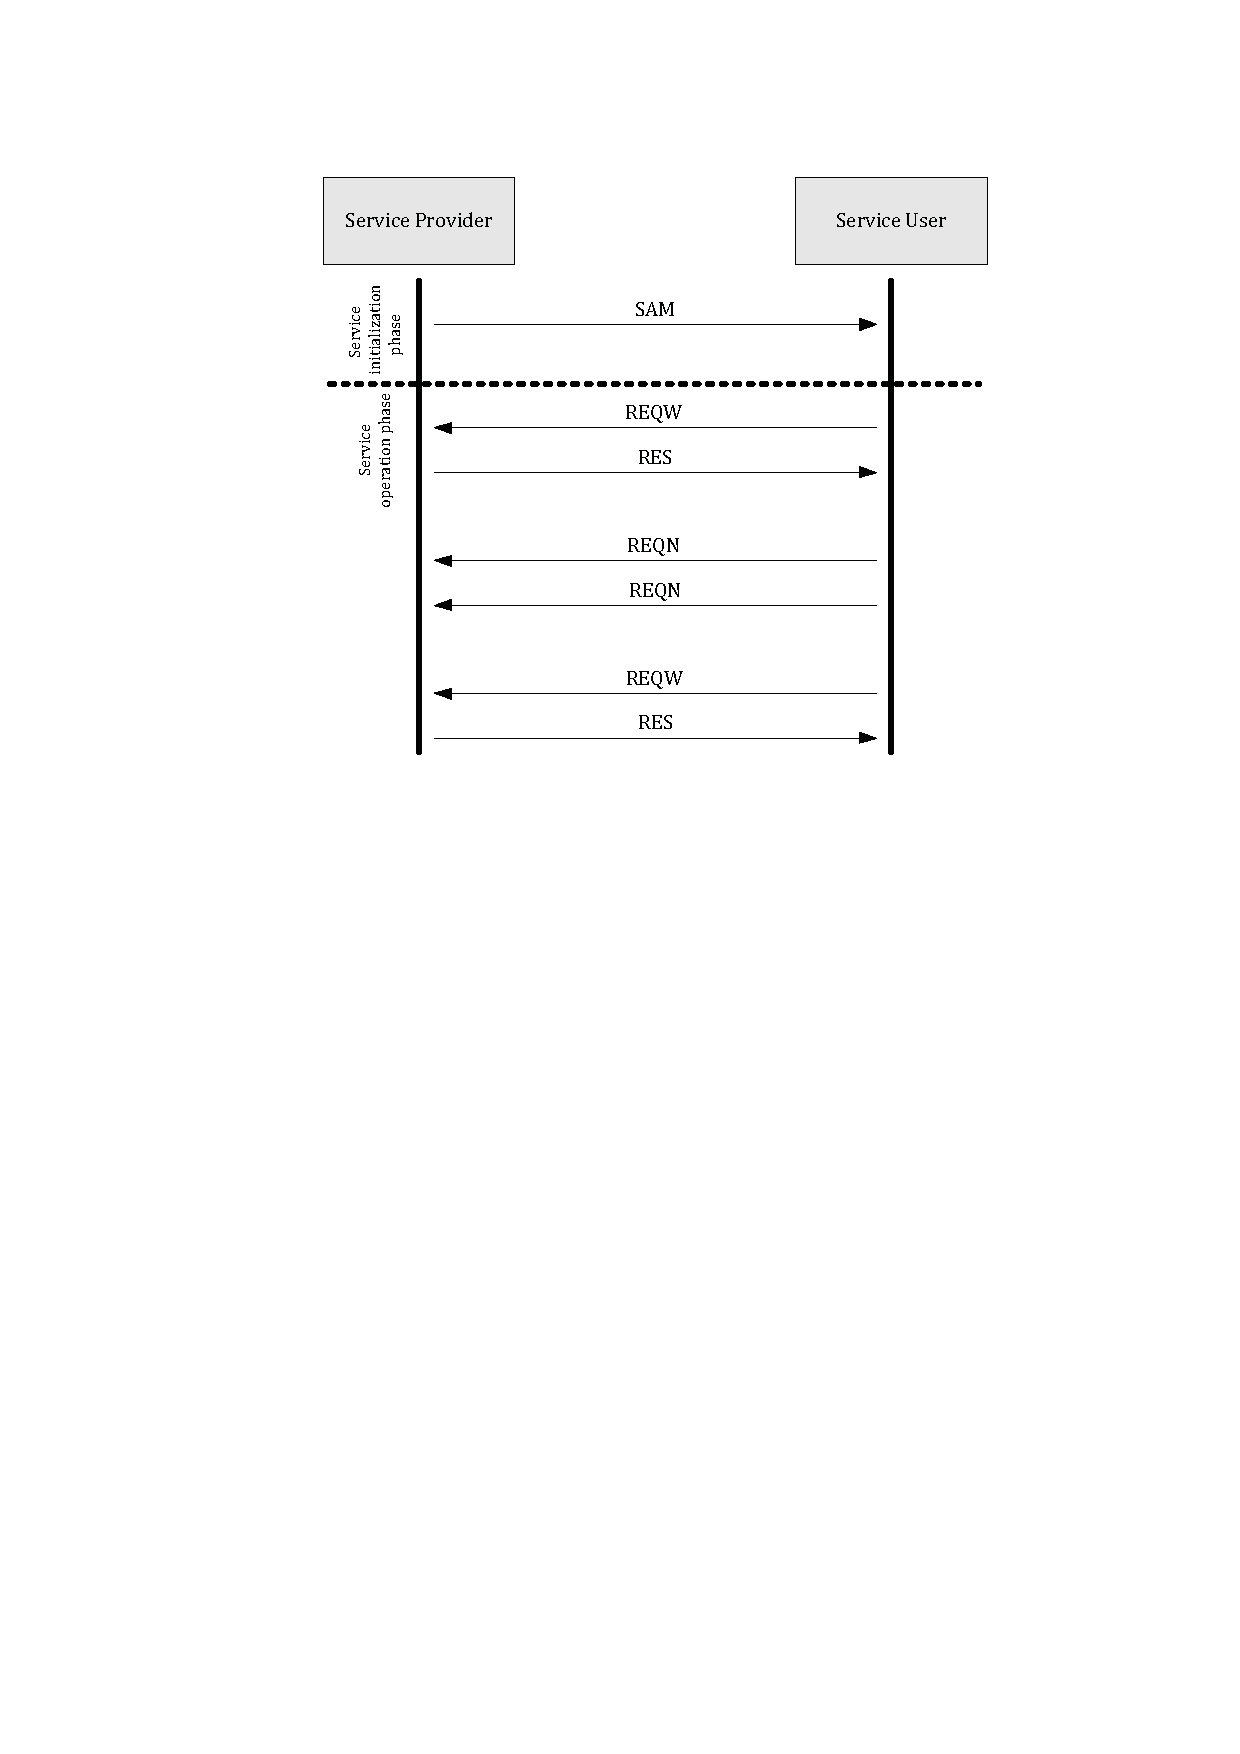
\includegraphics[width=0.45\textwidth]{content/images/02_architektur/serviceAdvertisementInit.pdf}}\qquad 
   \subfigure[Mit Bestätigung durch CTX]{ 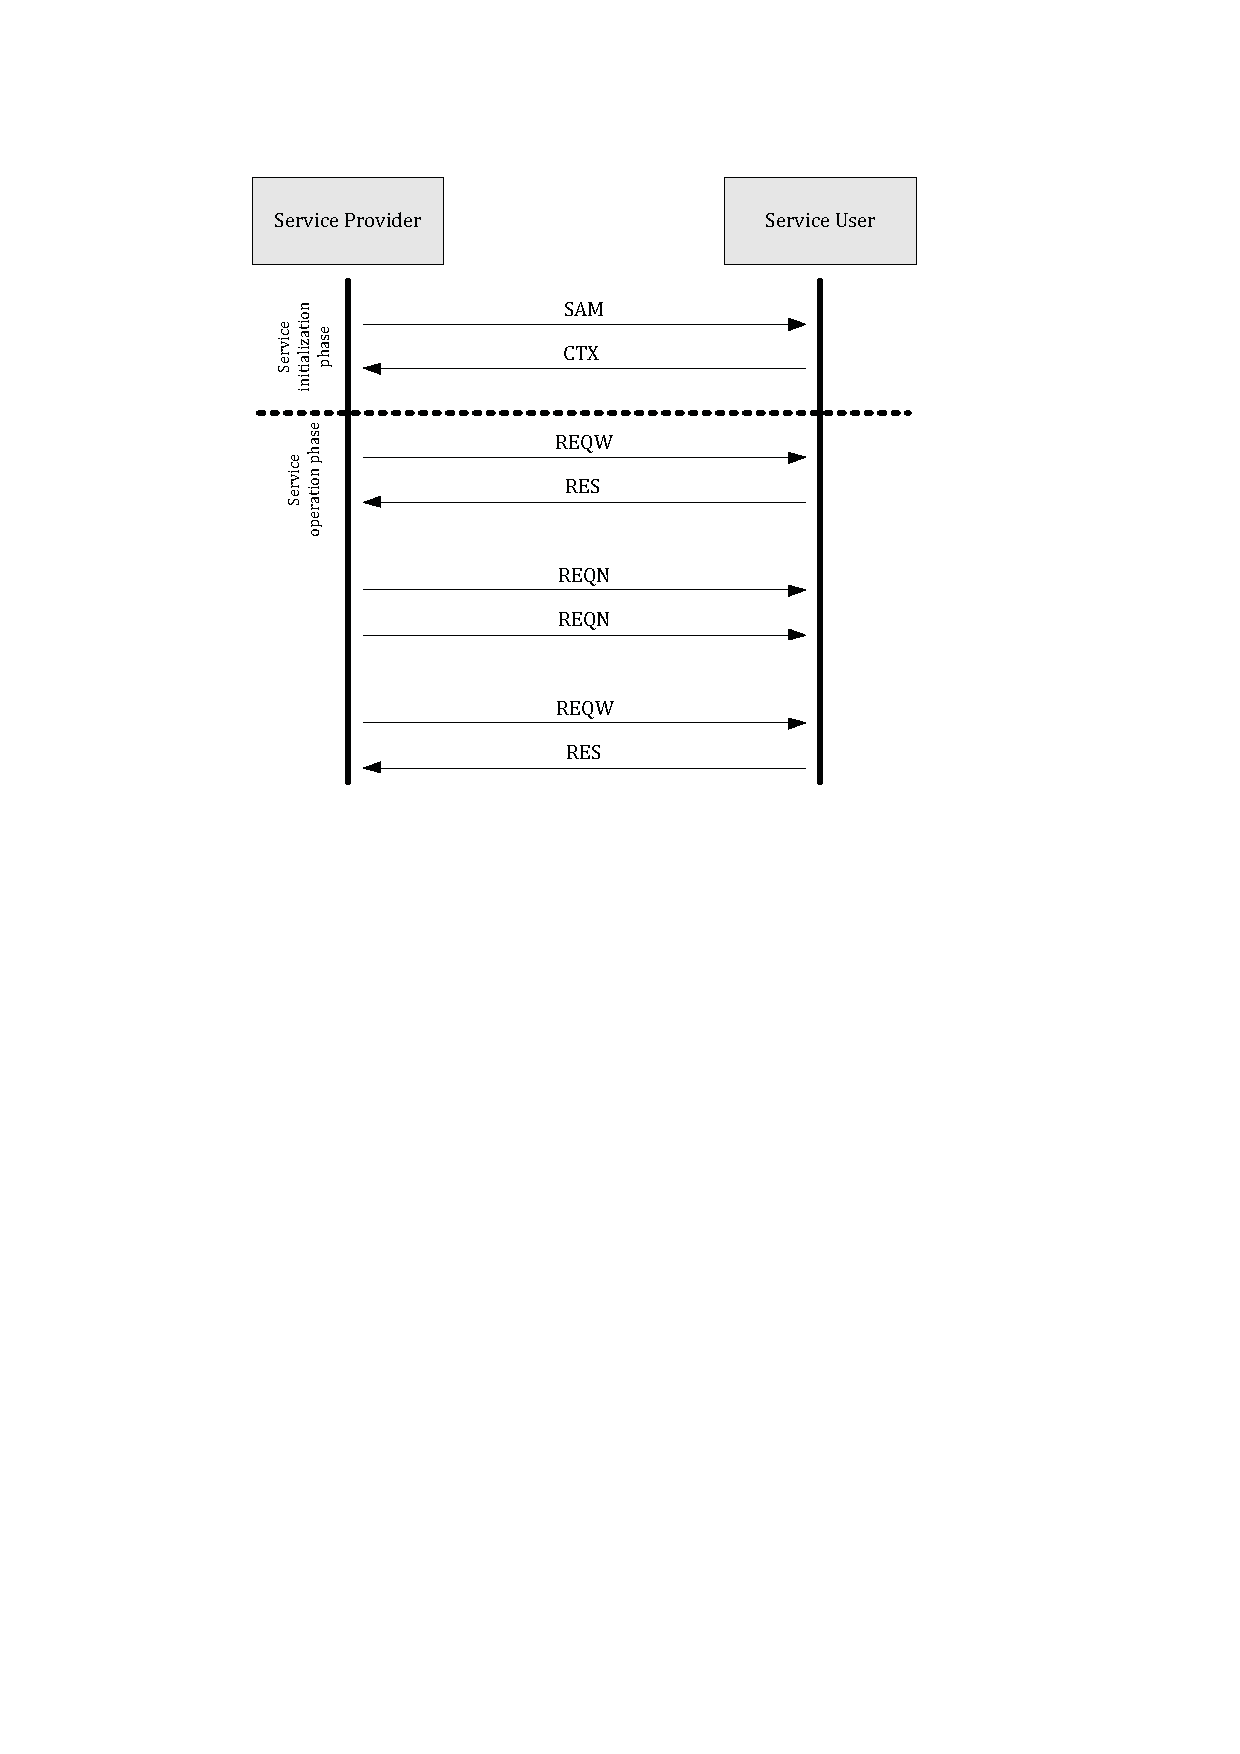
\includegraphics[width=0.45\textwidth]{content/images/02_architektur/serviceAdvertisementInitCTX.pdf}}
  \caption{Ablauf der Phasen des Fast Service Advertisement Protocol \cite{iso24102-5}} 
  \label{fig:architektur_ablaufPhasen}
\end{figure}
\todo{Prüfen, warum die Pfeile bei den Verbindungen genau umgekehrt sind}

In \autoref{fig:architektur_ablaufPhasen} wird der Ablauf der Phasen darstellt. Die einzelnen Schritte der Kommunikation bedeuten ausgeschrieben:
\begin{itemize}
	\item Request with no response expected (REQN)
	\item Request with response expected (REQW)
	\item Response to a request (RES)
\end{itemize}

Beschrieben in \cite{etsi102723-2}

\todo{Management Layer genauer beschreiben}

\todo{DCC genauer erklären und Text anpassen}

\subsubsection{Decentralizied Congestion Control\label{architektur_dcc}}
Congestion lässt sich aus dem Englischen mit Stau übersetzen. \ac{DCC} ist ein Mechanismus, der verhindern soll, dass Staus auftreten. Besonders bei \ac{ITS} Anwendungen kommt es auf zuverlässige und Übertragungswege an. Es werden hohe Anforderungen an die Verfügbarkeit und die Latenzen der Übertragungen gestellt. An Luftschnittstellen sind diese Anforderungen ohne eine Komponente wie \ac{DCC} kaum zu erfüllen. eine Der Standard \cite{etsi102687} definiert folgende Anforderungen an \ac{DCC}:
\begin{itemize}
	\item Eine faire Verteilung von Ressourcen und ein fairer Kanalzugriff zwischen allen \ac{ITS} Stationen in der gleichen Kommunikationszone
	\item Die Auslastung der Kanäle muss unter vordefinierten Werten bleiben. Dies muss durch eine periodische Messung sicher gestellt werden
	\item Reservierung von Kommunikationsressourcen für das Verbreiten von hoch priorisieren ereignisgesteuerten Nachrichten
	\item Schnelle Übernahme einer wechselnden Umgebung (busy / free radio channel)
	\item Die Änderungen in den Kontrollschleifen müssen in den definierten Grenzen bleiben
	\item Es muss den spezifischen Systemanforderungen, beispielsweise Zuverlässigkeit, entsprechen
\end{itemize}

Aus diesen Anforderungen lässt sich herauslesen, dass das Vermeiden von Staus durch mehrere Mechanismen realisiert wird. Eine wichtige Eigenschaft von \ac{DCC} ist, dass es im Management Layer angesiedelt ist. Diese Tatsache ermöglicht es \ac{DCC} seine Aufgaben parallel in mehreren Layern zu realisieren. Die \ref{fig:architektur_dccArchitektur} zeigt die Architektur von \ac{DCC}. Die Abbildung zeigt den \ac{ITS} Protokoll Stack in den die \ac{DCC} Komponenten und Interfaces eingezeichnet sind. Der Vorteil dass die Layer vernetzt sind ist, dass der Stau wirklich vermieden werden kann und nicht nur die Auswirkungen des Staus behandelt werden müssen. Ein Beispiel dafür ist, dass \ac{DCC} das Trafficaufkommen bereits im Network Layer an das Medium anpassen und einzelne Dienste priorisieren kann. IEEE 802.11 beispielsweise muss bei einer Überlast, bzw. einem Pufferüberlauf, Frames verwerfen. Dieses Verwerfen muss durch Protokolle höherer Layer abgefangen werden und führt aufgrund von Retransmissions zu höheren Latenzen und einer ingesamt höheren Netzwerkauslastung. 
\todo{Stimmt das mit dem Verwerfen eigentlich?}

\begin{figure}
	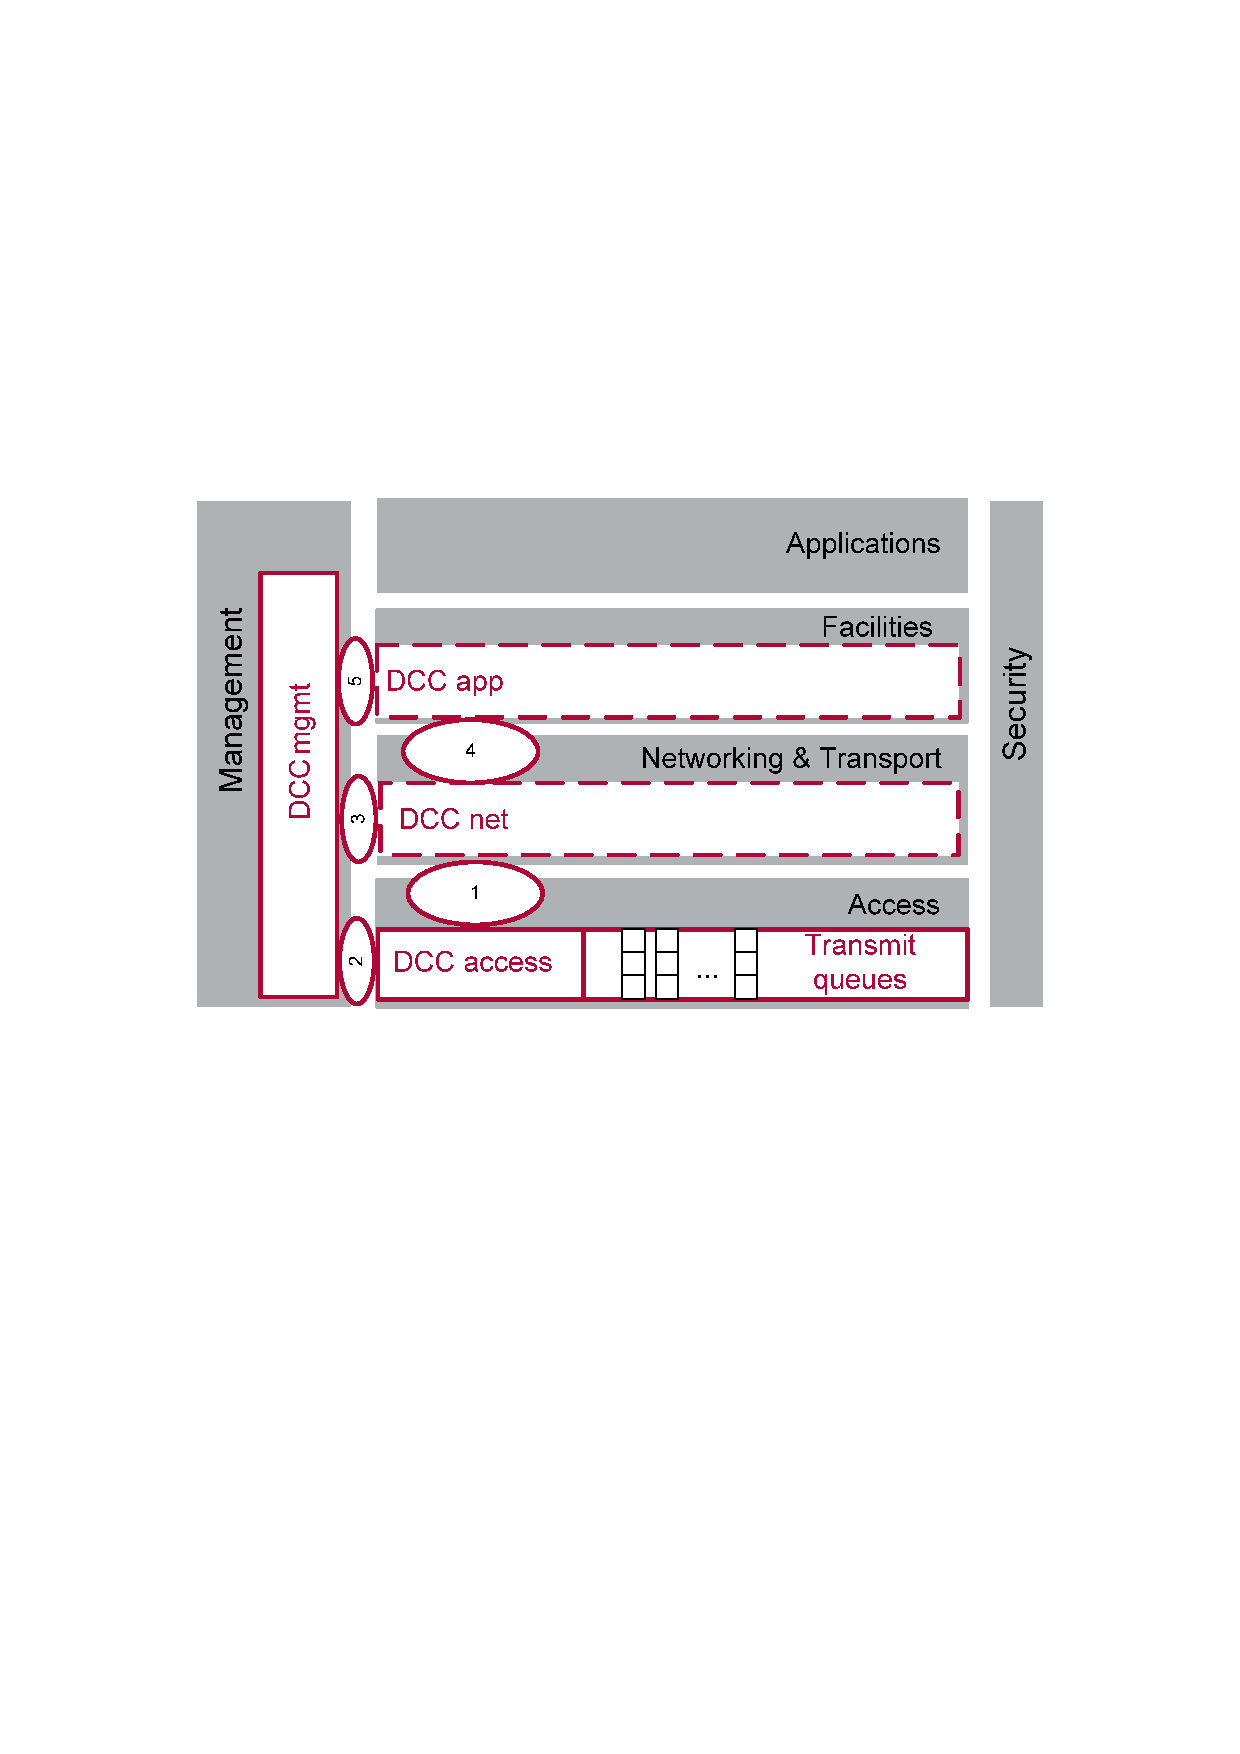
\includegraphics[width=0.75\textwidth]{content/images/02_architektur/dccArchitektur.pdf}
	\caption{Die Architektur von DCC \cite{etsi102687}}
	\label{fig:architektur_dccArchitektur}
\end{figure}

Für die Kommunikation mit mehreren Layern sind in der  \ac{DCC} Architektur vier Komponenten definiert. Die Komponenten sind mit den \ac{DCC} Interfaces verbunden, die selber auf den Interfaces der Layer zugeordnet werden. Die Komponenten werden in den Layern erklärt, in denen sie liegen. 

Die DCCmgmt Komponente ist im Management Layer angeordnet. Sie übernimmt dort die Cross Funktionalität und steuert die anderen Komponenten. Dazu hat sie Unterkomponenten.

Eine Unterkomponente der DCCmgmt Komponente ist die DCC\_CROSS\_Facilities. 



\subsubsection{CI/ITS-S application mapping}
\todo{Noch etwas über Application mapping schreiben}

\subsection{Security Layer \label{architektur_securityLayer}}
Der Security Layer ist ein Cross Layer der \ac{ITS} Architektur. Er sorgt für die Sicherheit im \ac{ITS} System. Er hat Interfaces in alle anderen Layer. 	\todo{Noch schreiben was der Security Layer genau macht} 
Der Standard \cite{en302665} beschreibt für den den Security Layer folgende Funktionalitäten:
\begin{itemize}
	\item Firewall und Angriff Management
	\item Authentifizierung, Autorisierung und Profilverwaltung
	\item Identitäts-, Krypto Schlüssel und Zertifikatsmanagement
	\item Eine allgemeine Sicherheit Informationsbasis (SIB)
	\item Hardware Security Module (HSM)
	\item Bereitstellung von Interfaces zu den anderen Layern, indem ihen Security Services angeboten werden
\end{itemize} 

\begin{figure}
	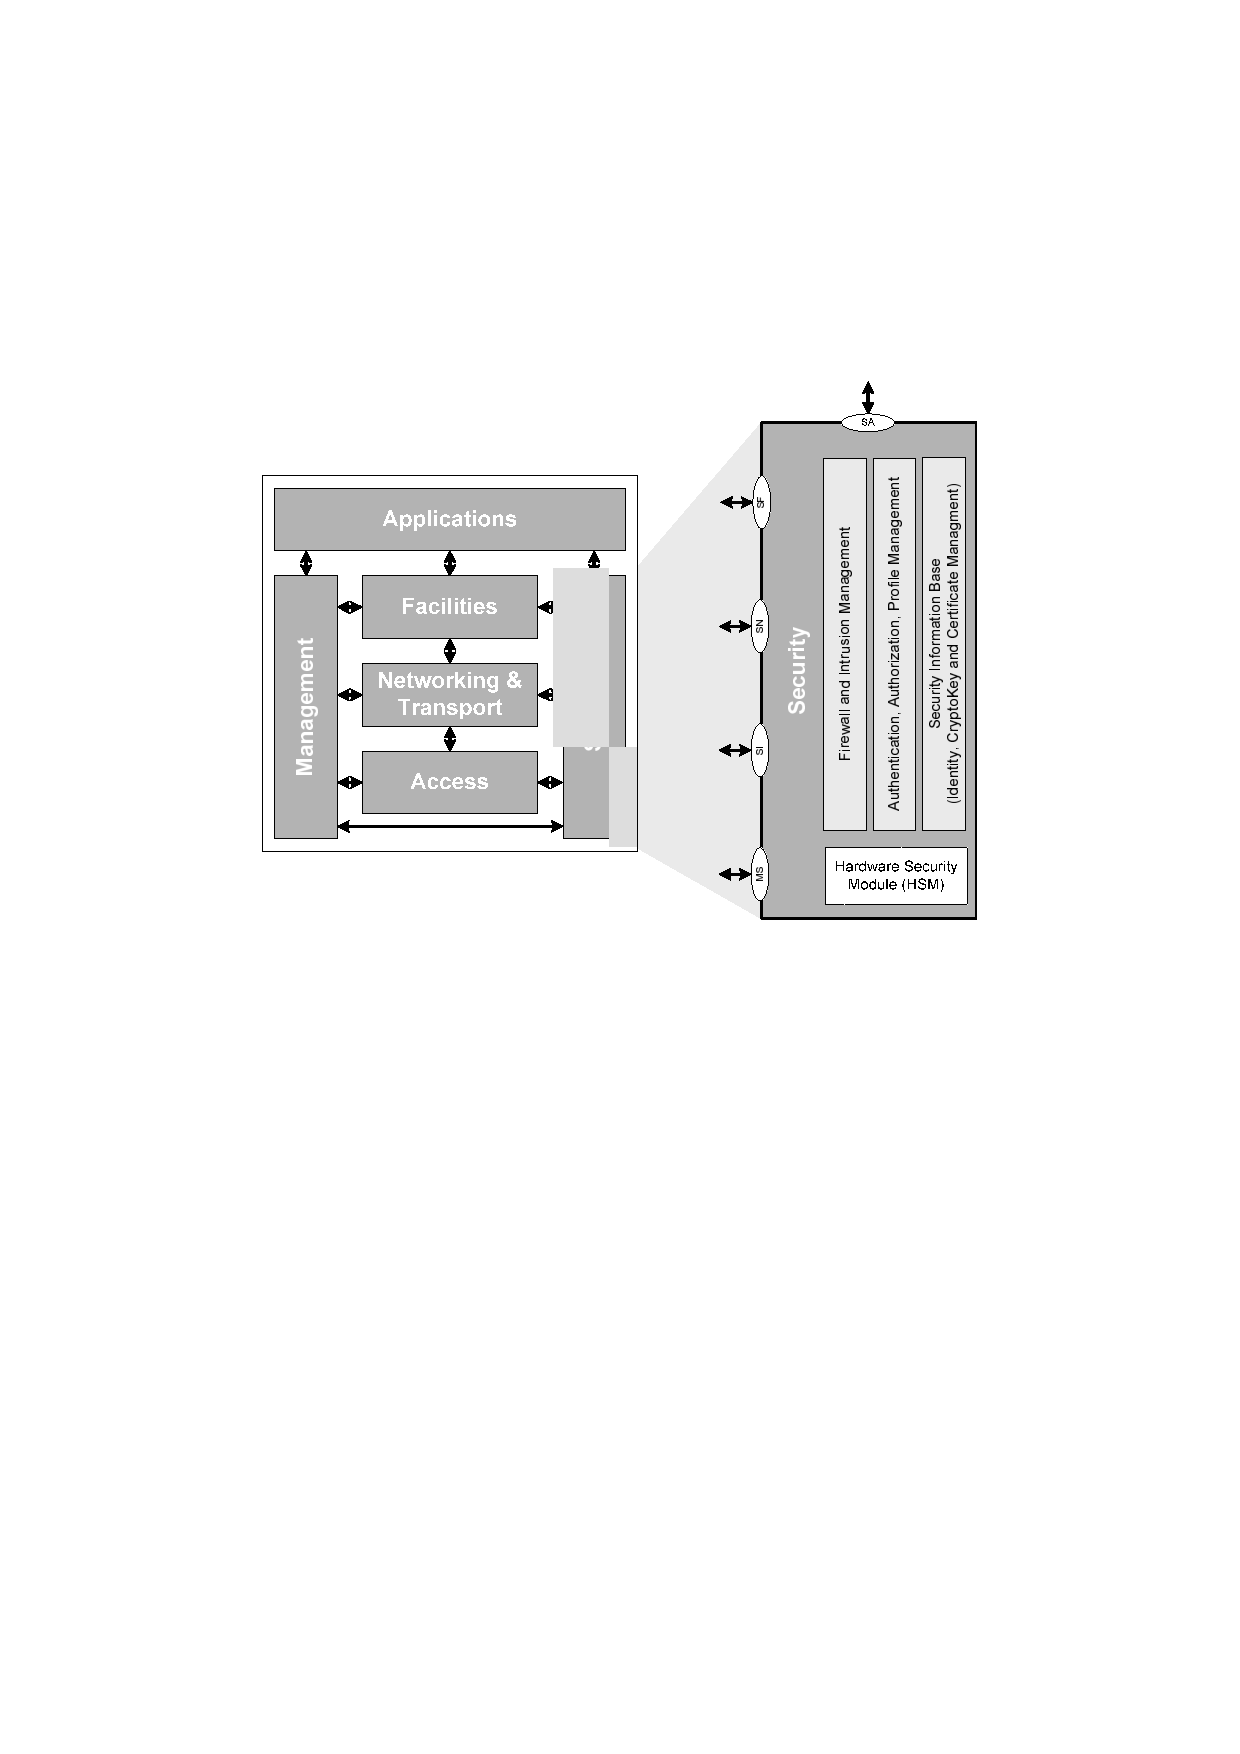
\includegraphics[width=0.75\textwidth]{content/images/02_architektur/securityLayer.pdf}
	\caption{Darstellung des Security Layers \cite{en302665}}
	\label{fig:architektur_securityLayer}
\end{figure}

\section{Data Security\label{architektur_dataSecurity}}
Der Begriff Security umfasst in \ac{ITS} verschiedene Bereiche der Sicherheit. Im \ac{ITS} Netz muss sichergestellt werden, dass die Nachrichten für die berechtigten Teilnehmer lesbar sind, für den unberechtigten Teilnehmer aber nicht. Dabei ist zu beachten, dass über \ac{ITS} sensible Daten verbreitet werden. Es muss neben dem Schutz gegen unbefugtes Lesen auch ein Mechanismus implementiert sein, der verhindert, dass falsche Informationen übertragen werden. Da die \ac{ITS} Architektur verschiedene Netzwerktypen \autoref{architektur_ueberblickNetzwerke} beinhaltet muss die Architektur auch ein Data Security Konzept beinhalten. Der Standard \cite{ts102940} spezifiziert dieses Konzept.  

\subsection{Angebotene Services}
 \begin{longtable}{| p{0.24\linewidth} | p{0.24\linewidth} | p{0.24\linewidth} |p{0.24\linewidth}|}
 \hline
 \textbf{Maßnahme} & & \textbf{Security Services} &  \\
 \cline{2-4}
 &\textbf{ First Level} & \textbf{Lower Level} & \textbf{Data Accessed}\\
 \hline
Include pseudonym in all V2V messages & Pseudonym Validation & & \\
 \hline
 Require an ITS-S to be authorized by an ITS authority before its messages are accepted by the ITS system & Obtain Enrolment Credentials & & Security Parameters (Authentication Keys)\\
 \hline
 Limit message traffic to V2I/I2V where possible & Obtain Enrolment Credentials & & Security Parameters (Authentication Keys) \\ 
 \cline{3-4}
 & & Authorization & Policy Database, Security Parameters (Authorization Ticket) \\
 \cline{3-4}
& & Establish Security Association & Security Parameters (Pseudonym, Encryption Keys) \\
 \cline{2-4}
 & Send Secured Message & Encrypt Outgoing Message & Security Parameters (Pseudonym, Encryption Key) \\
  \cline{3-4}
 &  & Authenticate Outgoing Message & Security Parameters (Pseudonym, Authentication Key) \\
 \cline{2-4}
 & Receive Secured Message & Decrypt Incoming Message & Security Parameters (Encryption Key) \\
  \cline{3-4}
 & & Validate Authentication on Incoming Message & Security Parameters (Pseudonym, Authentication Key) \\
 \cline{2-4}
 & Update Security Association & Remove Security Association & Security Parameters (Pseudonym, Encryption Key) \\
 \cline{3-4}
 & & Establish Security Association & Security Parameters (Pseudonym, Encryption Key) \\
 \cline{2-4}
 & Remove Enrolment Credentials & Authorization & Policy Database, Security Parameters (Authorization Ticket) \\
 \cline{3-4}
 & & Remove Security Association & Security Parameters (Pseudonym, Encryption Key) \\
 \hline
 Implement plausibility validation on incoming information & Validate Data Plausibility & Validate Dynamic Parameters & LDM \\
 \cline{3-4}
 & & Validate Timestamp & \\
 \cline{3-4}
 & & Validate Sequence Number &  \\
 \hline
 Include a non cryptographic checksum of the message in each message sent  & Insert Check Value & Calculate Check Value & \\
 \cline{2-4}
 & Validate Check Value & Calculate Check Value &  \\
 \hline
 Use broadcast time (Universal Coordinated Time - UTC - or GPS) to timestamp all messages & & Timestamp Message & \\
 \cline{3-4}
 & & Validate Timestamp & \\
 \hline
 Include a sequence number in each new message & & Insert Sequence Number & \\
  \cline{3-4}
 & & Validate Sequence Number & \\
 \hline
 Include an authoritative identity in each message and authenticate it & Validate pseudonym & & Security Parameters (Authentication Keys) \\
 \hline
Encrypt the transmission of personal and private data &  Send Encrypted Data & Encrypt Outgoing Message & Security Parameters (Encryption Keys) \\
\cline{2-4}
& Process Received Encrypted Data & Decrypt Incoming Message & Security Parameters (Encryption Keys) \\
\hline
Add an audit log to ITS stations to store the type and content of each message sent to and from an ITS-S &  Update Audit Log & Record Incoming ITS Messages& Audit Logs\\ \cline{3-4}
& & Record Outgoing ITS Messages & Audit Logs \\
\hline
Digitally sign each message using a Kerberos/PKI-like token & Sign Outgoing Message & Generate Signature & Security Parameters (Certificate, Keys) \\ 
\cline{3-4}
& &  Authorization & Policy database, Security Parameters (Authorization Ticket) \\
\cline{2-4}
& Verify Incoming Signed Message & Verify Signature & Security Parameters (Certificate, Keys) \\
\cline{3-4}
& & Authorization  & Policy database, Security Parameters (Certificate Status Information) \\
\hline
Use a pseudonym that cannot be linked to the true identity of either the user or the user's vehicle & Obtain Enrolment Credentials & Identification (authoritative identity provider) & Security Parameters (Pseudonym, Encryption Key) \\
\cline{2-4}
& remove Enrolment Credentials & Identification (authoritative identity provider) & Security Parameters (Pseudonym, Encryption Key)\\
\hline
Allow remote activation and deactivation of ITS-S & ITS-S Remote Management Report Misbehaving ITS-S & Authorization & Policy Database \\
\cline{3-4}
 & & Deactivate ITS Transmission & Security Parameters (Authorization Ticket) \\
 \cline{3-4}
& &  Activate ITS Transmission & Security Parameters (Authorization Ticket) \\
\cline{3-4}
& & Report Misbehaviour & Security Parameters (Authorization Ticket) \\
\hline 
\caption{Tabelle mit den Sicherheitsmaßnahmen \cite{ts102731}}
\label{tab:architektur_tabelleSicherheitsmassnahmen}
 
 \end{longtable}
\autoref{tab:architektur_tabelleSicherheitsmassnahmen} stammt aus dem Standard \cite{ts102731}. Dort werden die Maßnahmen zusammengefasst, die benötigt werden um sie zu erreichen. \glqq First Level\grqq~sind die Security Services, die direkt von den Anwendungen oder anderen Komponenten aufgerufen werden.  \glqq Lower Level\grqq~Services sind die, die von anderen Security Services aufgerufen werden.

\subsection{ITS Authoritative Hierarchy \label{architektur_itsAuthoriativeHierarchy}}
Die ITS Authoritative Hierarchy beschreibt, wer eine Rolle bei der Verwaltung der Sicherheit übernehmen kann. 

Die Hersteller von \ac{ITS} Stations unterstützen die regionalen Autorisierungsstellen indem sie die Identitäten der \ac{ITS} Stations verwalten. Dazu sollen sie ihnen während der Fertigung eine weltweite einzigartige Identität geben. Diese Identität soll  in Form eines Oktett Strings sein. Sie soll während der gesamten Lebensdauer gültig sein.\todo{Was will man da mit einem Oktett? Das sind 256 ITS Stations....  Original in ts 102 731: During the manufacturing process an ITS-S shall receive a globally unique canonical identity in the form of an octet string. It shall persist for the operational lifetime of the ITS-S.}
Neben der \ac{ID} müssen die \ac{ITS} Stations die Fähigkeit besitzen, die Verbindung mit mindestens einer Zertifikatsstelle und mindestens einer Autorisierungsstelle zu überprüfen.  Außerdem muss sie in der Lage sein, weitere Zertifikats- und Autorisierungsstelle hinzuzufügen.

Die Zertifikatsstelle, ist eine Einheit, die die Verwaltung der Zulassungszertifikate verantwortlich ist. Die Zertifikatsstelle werden verwendet um in Nachrichten zwischen \ac{ITS} Station und einer Security Management Einheit die \ac{ITS} Station als zugangsberechtigt auszuweisen. Das beinhaltet auch die Prüfung der Identität. Die Informationen zu der \ac{ITS} Station entnimmt die Zertifikatsstelle dem Zulassungszertifikat. Sie erstellt ein neues Zertifikat, und sendet es an die \ac{ITS} Station. Dieses Zertifikat bestätigt die Identität der \ac{ITS} Station und die der Zertifikatsstelle. Es findet lediglich die Bestätigung einer gültigen Identität statt,  auf die Identität selber können mit diesem Zertifikat keine Rückschlüsse gezogen werden. Wird eine \ac{ITS} Station als kompromittiert erkannt, informiert die Zertifikatsstelle die anderen Zertifikatsstellen. Dazu wird die eideutige \ac{ID} der \ac{ITS} Station den anderen Zertifikatsstellen mitgeteilt. Die \ac{ITS} Station bekommt so lange keine neuen Zertifikate, solange sie als kompromittiert bekannt ist.  

Die Autorisierungsstelle regelt den Zugang zu allgemeinen und speziellen Diensten. Um die Dienste der Autorisierungsstelle nutzen zu können muss die die Identität der \ac{ITS} Station durch ein Zertifikat einer Zulassungsstelle nachgewiesen werden. Die \ac{ITS} Station fragt bei der Autorisierungsstelle wegen der spezifischen Berechtigungen an. Die Anfragen werden \todo{An Authorization Authority weiterschreiben} Erkennt die Autorisierungsstelle, dass eine \ac{ITS} Station kompromittiert ist, so informiert sie die Zertifikatsstelle, von der die \ac{ITS} Station ihr Zertifikat hat. Ihr werden keine weiteren Tickets mehr mitgeteilt. Zusätzlich wird werden alle anderen \ac{ITS} Stations informiert, dass die Zertifikate ungültig sind.  


\subsection{Trust and Privacy Management}

Ein Aspekt der Data Security ist das Trust and Privacy Management. Der Standard \cite{ts102941} definiert für  den Begriff Privacy vier Schlüsselattribute:
\begin{itemize}
	\item Anonymity
	\item Pseudonymity
	\item Unlinkability
	\item Unobservability
\end{itemize}

Der Begriff anonymity bedeutet übersetzt Anonymität und erklärt sich von alleine. Der Begriff bedeutet, dass jemand anonymes keine Identität zugeordnet werden kann. Ein Bespiel hierfür ist eine völlig zufällige Nummer, die anstelle der Identität angegeben wird. Ihr kann keine Identität zugeordnet werden. Da einigen Services der \ac{ITS} Architektur eine Authentifizierung zu Grunde liegt ist eine vollständige Anonymisierung nicht möglich. Aus diesem Grund gibt es die drei anderen Schlüsselwörter. 

Pseudonymity bedeutet übersetzt Pseudonymisierung.  Pseudonymisierung wird oft mit Anonymisierung verwechselt, bedeutet aber etwas Anderes. Hinter etwas pseudonymisiertem steht eine Identität, die durch das  pseudonymisierte ersetzt wurde. Ein Beispiel hierfür ist die Matrikelnummer eines Studenten. Einem Angreifer, ohne die Möglichkeit, die Matrikelnummer dem Namen eines Studenten zuzuordnen, ist der Student gegenüber anonym. Besteht die Möglichkeit jedoch kann der Matrikelnummer sehr wohl eine Identität zugeordnet werden. Der Nachteil von Pseudonymen ist, dass sie wertlos sind, sobald ein Teil des Systems kompromittiert wurde. In \ac{ITS} wird die  Psyeudonymität erreicht, indem nur temporäre Kennungen von \ac{ITS} Stations verwendet werden.

Ein weiterer Nachteil von Pseudonymen ist, dass mit der erfassten Datenmenge die Chance steigt, von ihnen auf eine Identität zu schließen. Wird die Nutzung eines Pseudonyms verfolgt können die Aktivitäten miteinander Verlinkt werden. Dadurch kann aus dem Pseudonym eine neue Identität werden, von der Rückschlüsse auf die Identität hinter dem Pseudonym getroffen werden können. Es kann aber auch die Identität aus dem Verhalten ermittelt werden. Um bei dem Beispiel mit dem Studenten zu bleiben, kann über ihn, bzw. seine Matrikelnummer, ein Bewegungsprofil erstellt werden, das  einzigartig ist. Wird die Matrikelnummer für das Einschreiben in Kurse genutzt kann nach genug Einschreibungen das Studienfach und das Studiensemester ermittelt werden. Diese Sammlung nennt man Verkettung von Daten. Das Schlüsselwort unlinkability fordert, dass eine \ac{ITS} Station nicht verkettbar ist. In \ac{ITS} wird die Verkettbarkeit verhindert, indem die Verwendung von nicht, oder kaum, veränderter Informationen. Damit kann Verbindungen von \ac{ITS} Stations nicht anderen Verbindungen zugeordnet werden.

Unobservability bedeutet, dass der Nutzer eine Ressource nutzen kann, ohne dass andere Nutzer, oder Dritte, feststellen können, dass dieser Dienst genutzt wird.

Durch die Beachtung dieser Schlüsselwörter bei der weiteren Spezifikation und der Implementierung von \ac{ITS} wird der Datenschutz bereits im Vorfeld beachtet. 

Neben dem Datenschutz muss im \ac{ITS} System aber auch eine Zugangskontrolle realisiert werden. Die Zugangskontrolle teilt sich in zwei Bereiche auf: Die Berechtigung, das \ac{ITS} System als Ganzes zu nutzen und die Berechtigung, einzelne Services und Anwendungen zu nutzen. Die Prüfung der Identitäten wird über Zertifikate und Public-Key Verfahren realisiert. Zur Verteilung der Berechtigungen werden im Standard \cite{ts102731} definiert.

\subsection{ITS Security Serivces}
Bei den in \ac{ITS} versendeten Nachrichten müssen aus Sicht der Sicherheit drei verschiedene Typen betrachtet werden. 

Der erste Typ ist die \glqq Individual public message\grqq~Dieser Typ wird per Broadcast an andere \ac{ITS} Stations versendet. Da es sich um eine Broadcast Nachricht handelt, ist eine Verschlüsselung nicht nötig. Um zu verhindern, dass mit dieser Nachricht Fehlinformationen übertragen werden muss sie lediglich signiert werden. Der Standard \cite{ts102731} nennt für diesen Typ von Nachricht die Schlagwörter: authorization, authentication und integrity. Damit wird ausgedrückt, dass die sendende \ac{iTS} Station im System legitimiert sein muss, die Nachricht wird als Schutz gegen Verfälschungen und fehlerhafte Nachrichten von Angreifern aber signiert.

Der zweite Typ ist die \glqq    Individual private message\grqq~. Sie wird an eine bestimmte \ac{ITS} Station verschickt. Da hier kein Broadcast vorliegt, macht es auch Sinn diese Nachricht zu verschlüsseln. Der Standard nennt zu diesem Nachrichtentyp die Schlüsselwörter require authorization, authentication, integrity, privacy und confidentiality. Diese Schlüsselwörter erweitern die Schlüsselwörter der \glqq Individual public message\grqq~um den Faktor, dass der Inhalt von Dritten nicht mitgelesen darf. Aus diesem Grund findet zusätzlich eine Verschlüsselung der Nachricht statt.

Als drittes sind die \glqq Security Associations\grqq zu nennen. Sie werden zwischen zwei oder mehreren \ac{ITS} Stations aufgebaut und beinhalten einen Satz von Krypto Algorithmen, Schlüsseln und andere private und öffentliche Parameter. Sie werden genutzt um eine Ende zu Ende Verbindung aufzubauen.  Der Standard nennt die Schlüsselwörter confidentiality, authentication und integrity.  Diese entsprechen prinzipiell den Schlüsselwörtern der \glqq    Individual private message\grqq. Diese Verbindungen können auf andere autorisierte Teilnehmer dupliziert werden. Jeder Teilnehmer kann mehrere sichere Verbindungen haben. Wenn de sichere Verbindung aufgebaut wird, sollen die Zertifikate und die Kryptowerkzeuge die mit den sicheren Verbindungen verknüpft sind genutzt werden. Die sichere Verbindung soll ab und zu neu verhandelt werden. 

Die beschriebenen Nachrichtentypen benötigen Zertifikate. In \ac{ITS} sind zwei verschiedne Sorten von Zertifikaten definiert. Es gibt ein \glqq  authorization ticket\grqq. Es ist als ein Datenobjekt beschrieben, dass bestätigt, dass der gültige Inhaber berechtigt ist, verschiedene Aktionen auszuführen. Es wird von der ITS Autorisierungsstelle\ref{architektur_itsAuthoriativeHierarchy} ausgestellt. Die zweite Sorte Zertifikat ist das \glqq enrolment credential\grqq. Es wird als ein Datenobjekt das im Nachrichtenaustausch zwischen \ac{ITS} Stationen und Security Einheiten genutzt und beweist, dass der gültige Inhaber berechtigt ist, authorization tickets anzufragen. Es wird von der Zertifikatsstelle ausgestellt. Die folgenden Abschnitte erläutern wie die Verarbeitung der Zertifikate statt findet.

\subsubsection{Enrolment Credentials}
Enrolment Credentials können ausgestellt, erneuert und gelöscht werden. 

Das Anfordern eines enrolement credentials geschieht in zwei Schritten. Der erste Schritt ist, dass eine \ac{ITS} Staion merkt, dass sie sich an der \ac{ITS} Infrastruktur anmelden muss. Dieser Schritt löst die Anmeldungsanfrage an die \ac{ITS} Infrastruktur aus.
\todo{Ausformulieren}

\todo{Evtl. noch Abschnitt über die Interfaces zu den anderen Layern 302 665 Informative Quellen}




\subsection{Access Control}

\section{Verwendete Protokolle}




